\documentclass[11pt,oneside,letterpaper]{article}

% graphicx package, useful for including eps and pdf graphics
\usepackage{graphicx}
\DeclareGraphicsExtensions{.pdf,.png,.jpg}

% basic packages
\usepackage{color} 
\usepackage{parskip}
\usepackage{float}

% text layout
\usepackage{geometry}

\geometry{textwidth=15cm} % 15.25cm for single-space, 16.25cm for double-space
\geometry{textheight=22cm} % 22cm for single-space, 22.5cm for double-space

% helps to keep figures from being orphaned on a page by themselves
\renewcommand{\topfraction}{0.85}
\renewcommand{\textfraction}{0.1}

% bold the 'Figure #' in the caption and separate it with a period
% Captions will be left justified
\usepackage[labelfont=bf,labelsep=period,font=small]{caption}

% review layout with double-spacing
%\usepackage{setspace} 
%\doublespacing
%\captionsetup{labelfont=bf,labelsep=period,font=doublespacing}

% cite package, to clean up citations in the main text. Do not remove.
\usepackage{cite}
%\renewcommand\citeleft{(}
%\renewcommand\citeright{)}
%\renewcommand\citeform[1]{\textsl{#1}}

% Remove brackets from numbering in list of References
\renewcommand\refname{\large References}
\makeatletter
\renewcommand{\@biblabel}[1]{\quad#1.}
\makeatother

\usepackage{authblk}
\renewcommand\Authands{ \& }
\renewcommand\Authfont{\normalsize \bf}
\renewcommand\Affilfont{\small \normalfont}
\makeatletter
\renewcommand\AB@affilsepx{, \protect\Affilfont}
\makeatother

% notation
\usepackage{amsmath}
\usepackage{amssymb}
\newcommand{\virus}{\mathbf{x}}						% virus coordinate
\newcommand{\serum}{\mathbf{y}}						% serum coordinate
\newcommand{\viruses}{\mathbf{X}}					% set of virus coordinates
\newcommand{\sera}{\mathbf{Y}}						% set of serum coordinates
\newcommand{\ve}{v}									% virus avidity
\newcommand{\se}{s}									% serum potency
\newcommand{\ves}{\mathbf{v}}						% set of virus avidities
\newcommand{\ses}{\mathbf{s}}						% set of serum potencies
\newcommand{\point}{f_{\scriptscriptstyle \vert}}	% point likelihood
\newcommand{\threshold}{f_{\textstyle \lrcorner}}	% threshold likelihood
\newcommand{\interval}{f_{\sqcup}}					% interval likelihood
\newcommand{\mdssd}{\varphi}						% MDS standard deviation
\newcommand{\virussd}{\sigma_x}						% virus / diffusion standard deviation
\newcommand{\serumsd}{\sigma_y}						% serum standard deviation
\newcommand{\drift}{\beta}							% drift / advection
\newcommand{\tree}{\tau}							% phylogeny
\newcommand{\vn}{n}									% number of viruses
\newcommand{\sn}{k}									% number of sera
\newcommand{\normal}{\mathcal{N}}					% normal distribution
\newcommand{\bwithin}{\beta_w}		% within clade drift coefficient
\newcommand{\bsister}{\beta_s}		% sister clade drift coefficient
\newcommand{\bother}{\beta_t}			% across clade drift coefficient
\newcommand{\incclade}[1]{y_\mathrm{#1}}
\newcommand{\driftclade}[1]{x_\mathrm{#1}}
\setlength{\arraycolsep}{2pt}
\newcommand{\smalltwomatrix}[2]{\scriptsize \Big( \begin{matrix} #1 \\ #2 \end{matrix} \Big)}				% pretty inline matrix 
\newcommand{\smallfourmatrix}[4]{\scriptsize \Big( \begin{matrix} #1 & #2 \\ #3 & #4 \end{matrix} \Big)}	% pretty inline matrix 
\newcommand{\twomatrix}[2]{\left( \begin{matrix} #1 \\ #2 \end{matrix} \right)}								% pretty inline matrix 
\newcommand{\fourmatrix}[4]{\left( \begin{matrix} #1 & #2 \\ #3 & #4 \end{matrix} \right)}					% pretty inline matrix 


%%%http://www.oxfordjournals.org/our_journals/molbev/general_author_guidelines.html%%%

%%%Cover Page
%%%On the top right corner of the first page, clearly indicate if the submission is intended as an Article, Letter, Brief Communication, Perspective, Protocol, or Review. For Articles and Letters, clearly indicate whether the work best fits in the Discoveries, Methods, or Resources section of MBE. The cover page should contain a brief and informative Title that should be accessible to general readers of MBE. Below the title, list all author names and their current affiliations, including institution(s) at which research was done. Then, list the name and e-mail address of the corresponding author.%%%



%%% Theoretical and methodological reports need to clearly demonstrate the robustness and practical utility of the advanced methods using computer simulations and example data analysis. %%%

%%%Articles must clearly describe how the advances will broaden the application scope or significantly accelerate the pace of biological discovery.%%%

% Articles - Methods       (Need to include it in the top right:    )

%%% TITLE %%%
\title{\vspace{1.0cm} \Large \bf 
%Clustering viruses using Antigenic Data and Phylogeny
Detailed antigenic dynamics of influenza virus revealed by Bayesian phylogenetic clustering
}

\author[1]{Charles Y K Cheung}
\author[2]{Marc A Suchard} 
\author[3,4]{Andrew Rambaut}
\author[1]{Trevor Bedford}

\affil[1]{Vaccine and Infectious Disease Division, Fred Hutchinson Cancer Research Center, Seattle, WA, USA}
\affil[2]{Departments of Biomathematics and Human Genetics, David Geffen School of Medicine at UCLA and Department of Biostatistics, UCLA Fielding School of Public Health, University of California, Los Angeles, California, U.S.A}
\affil[3]{Institute of Evolutionary Biology, University of Edinburgh, Ashworth Laboratories, Edinburgh, UK and Fogarty International Center, National Institutes of Health, Bethesda, MD, USA}
\affil[4]{Fogarty International Center, National Institutes of Health, Bethesda, MD, USA}


% Corresponding author: Trevor Bedford (trevor@bedford.io)   %need to include it in

\date{}


\begin{document}

\maketitle


\newpage


%%%Format: Articles have an abstract of up to 250 words. This is followed by sections (in order) with headings: Introduction, Results, Discussion, and Materials and Methods. Results and Discussion may be combined. Subsections are allowed throughout. For articles describing new or improved methods and resources, authors should add a section entitled New Approaches after the Introduction. This section should clearly and succinctly present the new or improved methods or approaches, with extensive details provided in the Materials and Methods section, if necessary (See General Author Guidelines for all other information on manuscript preparation).%%%


%%% ABSTRACT %%%
\begin{abstract}

%%%  can have 250 words - currently 249 words %%%
Each year, infection by seasonal influenza viruses cause over 250,000 deaths. 
Vaccination remains the most effective way to limit epidemic spread. 
To select a vaccine strain, the World Health Organization uses antigenic cartography, a technique based on multidimensional scaling, to analyze serological data from hundreds of virus isolates. 
Here, we extend this method to enable systematic clustering of viruses into discrete antigenic phenotypes. 
The method explicitly leverages information from virus phylogeny to relate genotype evolution to the emergence of major antigenic phenotypes. By relating these two processes, the method probabilistically infers branches associated with antigenic transitions. 
This new method extends a recently introduced Bayesian multidimensional scaling technique for antigenic cartography to capture uncertainty in clustering and cartographic location.
Posterior distributions were computed using Markov chain Monte Carlo with model-specific proposals to address the challenge of efficient mixing. 
In our considered setting, results from simulations suggest that our method can detect antigenic clusters with high sensitivity ($\sim$90\%) even when the proportion of missing measurements is high (90\%).
Here, we analyze several decades of historical A/H1N1 and A/H3N2 antigenic data to infer circulating antigenic phenotypes. 
In A/H3N2, our method identified XXX clusters with high confidence and estimated the rate of antigenic transitions to be XXX events per lineage per year.
We also estimate the distribution of antigenic transition sizes and the degree of co-circulation of competing antigenic phenotypes.
We believe that this method may have utility in identifying emerging antigenic phenotypes and thus may facilitate surveillance efforts.

\hfill

%Key words: Markov chain Monte Carlo, Bayesian, phylogenetics, clustering, virus evolution, antigenic drift %these are two statistically centric. good for JSM but not appropriate for MBE

%% Older version %%
%%%Antigenic cartography is an important statistical tool that the World Health Organization uses to analyze antigenic data to assist policy makers in deciding whether to update Influenza vaccine strain. Here, we extended this tool to enable systematic clustering of viruses into antigenic phenotypes. Motivated by an existing Bayesian nonparametric method that uses viral sequences to assist with clustering, we devised a complementary method that can relate the evolution of viral sequences to the emergence of major antigenic phenotypes by explicitly leveraging an inferred phylogenetic tree. Our method builds on a recent Bayesian Multi-dimensional Scaling method that allows us to capture uncertainty in the inference. Via this framework, we used Bayesian Stochastic Search Variable Selection on tree nodes to probabilistically infer branches associated with major antigenic changes. We developed model-specific proposals to address the challenge of mixing when performing computation using the Markov chain Monte Carlo. We analyzed the H3N2 data and achieved high concordance with previously defined clusters while identifying additional antigenic clusters that might have been overlooked.%%%

\end{abstract}

%%% IMPACT %%%
% Combined evolutionary and antigenic analysis shows that human influenza viruses differ dramatically in rates of antigenic drift and these rates significantly impact seasonal incidence patterns.

\pagebreak

%%% INTRODUCTION %%%
\section*{Introduction}

Antigenically variable pathogens such as influenza viruses are a major disease burden worldwide. 
These pathogens have the ability to constantly evade immunity, allowing them to re-infect hosts with prior exposure or vaccination. 
One notable example is the A/H3N2 influenza virus, in which new antigenic phenotypes frequently emerge and displace existing variants \cite{smith_mapping_2004, bedford_integrating_2014}.
Genetic mutations in the hemagglutinin (HA) gene, which encodes a surface protein that allows the virus to enter a host cell, enable this virus strain to escape recognition by antibodies previously elicited to target this strain from a previous infection. 
Understanding the relationship between genotype and antigenic evolution is an important task from both public health and evolutionary and molecular biological perspectives.
%genetic drift, antigenic drift.
% selective pressure 

%Question: go into explicit details about how we measure antigenic variation in the introduction? Why is it important, or is it not?
Serological data provides important information about the antigenic phenotype of influenza viruses \cite{smith_mapping_2004}. 
In a typical experiment of influenza virus, a ferret is challenged by a reference virus, such as a vaccine strain.
Subsequently, the ferret produces antibodies to neutralize the challenge virus. 
Then, the experimenter would extract blood serum containing these antibodies to perform a hemagglutination inhibition (HI) assay  on a panel of viruses that are of current interest. 
A high titer value corresponds to strong reactivity between antibodies in the ferret serum and the tested virus, as would be expected when this test virus is homologous to the reference serum.
On the other hand, a low titer value suggests that this test virus is antigenically distinct from the reference strain. 
In recent decades, the World Health Organization (WHO) has collected titer measurements from large panels of viruses and sera \cite{smith_mapping_2004, russell_global_2008}. 
As tables of these measurements accumulate, extracting, summarizing, and interpreting this antigenic data to understand historical and emerging antigenic variation has become an increasingly challenging task. % TB: great sentence!

Since its introduction, antigenic cartography \cite{smith_mapping_2004, cai_computational_2010} has become an indispensable tool used to study antigenic variation in influenza virus and other antigenically variable pathogens such as foot and mouth disease virus, enteroviruses, and HIV \cite{smith_mapping_2004, jong_antigenic_2007, ludi_antigenic_2014, debbink_withinhost_2014, frost_mapping_2013}.
Antigenic cartography is a dimensionality-reduction technique based on multidimensional scaling (MDS) to create intuitive and interpretable two
dimensional antigenic maps. 
An antigenic map summarizes the relationship between viruses and sera.
In influenza viruses, HI titer is inversely proportional to Euclidean distance between viruses and sera.
Viruses that are close together on an antigenic map are expected to share similar antigenic phenotypes. 

Identifying distinct antigenic phenotypes is an important task for monitoring the evolution of antigenic phenotypes and for making decisions related to vaccine strain selection in humans and animals \cite{smith_mapping_2004, fouchier_use_2010}.
Most commonly, clustering viruses into antigenic phenotypes are performed by manual classification or by performing $k$-means clustering on the antigenic map \cite{smith_mapping_2004}. 
In the presence of measurement noise, non-trivial relationships between viruses and sera, and missing data \cite{cai_computational_2010}, it could be difficult to interpret clusters from tables of antigenic data or by even by visually inspecting the antigenic map. 
Therefore, systematic integration of other information such as the viral sequences could enable a more informative inference of major antigenic clusters.
Recently, Cybis et al. \cite{cybis_bayesian_2015} proposed a method to perform probabilistic clustering based on a recently introduced Bayesian multidimensional scaling method \cite{oh_bayesian_2001} that allows integration of viral sequences \cite{bedford_integrating_2014}. 
This method offers two main contributions. 
First, the Bayesian framework allows antigenic clustering to take into account uncertainty in the inference of antigenic locations \cite{bedford_integrating_2014}.
Second, by integrating sequence data via the number of substitutions between each pair of sequence modeled using the distance-dependent Chinese restaurant process \cite{blei_distance_2011}, viruses that are more closely related would \textit{a priori} be more likely to be classified into the same clusters. 
These existing methods, however, do not provide a direct mapping between genetic and antigenic evolution. 
As antigenic evolution arises from genetic evolution, we believe that a clustering method that explicitly models the connection between these two components would further contribute to the understanding of this link and result in a more powerful genotype-phenotype model.

\begin{figure}[h]
	\centering		
	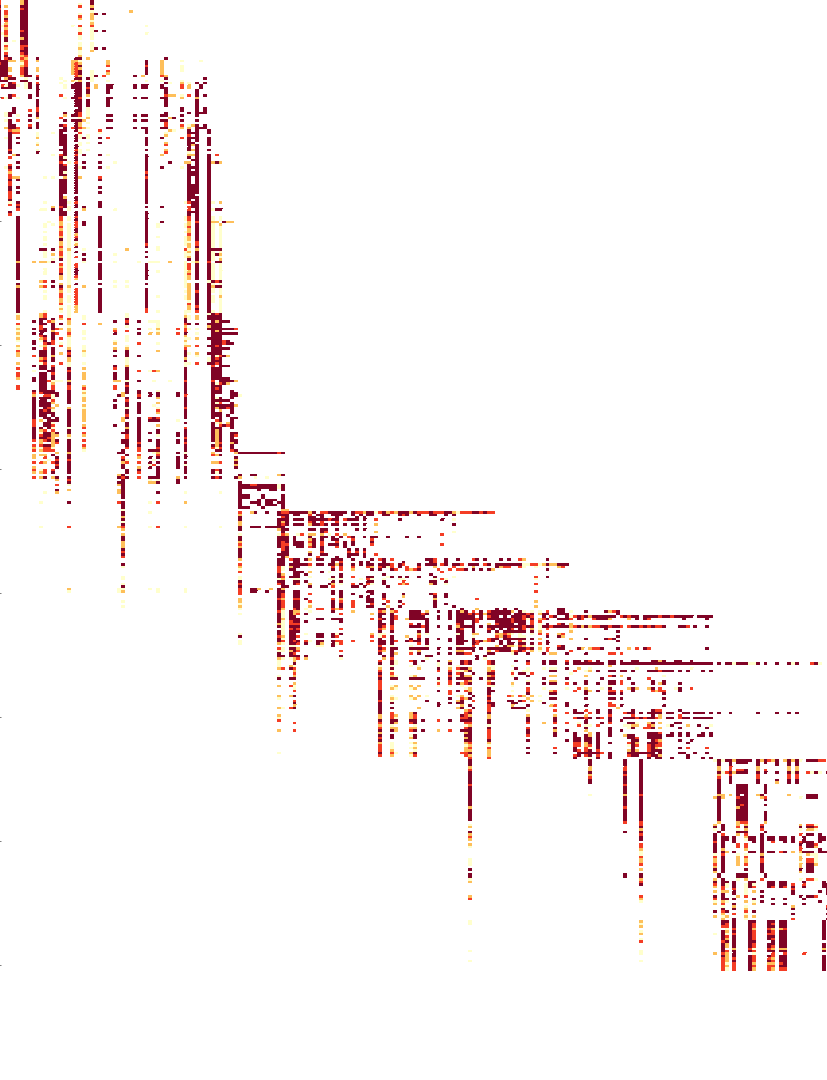
\includegraphics[width=0.7\textwidth]{figures/custom/heatmapFromBedfordData-cropped}
	\caption{\textbf{H3N2 hemagglutination inhibition assay titers. [WILL WORK ON IT]} 
		} 
	\label{H3N2titer} 
\end{figure}

%one reason we spent so much time to analyze this data is because this dataset is very important from the public health perspective.
Here, we introduce a new method for clustering viruses that relates genetic and antigenic evolution. 
Our work extends the original model for antigenic cartography \cite{smith_mapping_2004} and the Bayesian multidimensional scaling approach \cite{bedford_integrating_2014} to succinctly summarize the overall relationship between viruses and sera from the HI data in lower dimension.
This method, which is intuitive and philosophically simple, offers two important advantages over existing methods. 
First, by leveraging an inferred viral phylogeny that provides information about the evolutionary relationship among viruses, we are able to probabilistically infer the branches in the phylogeny where the most important antigenic transition occurs. 
Second, by incorporating phylogeny explicitly, we can estimate other interesting parameters such as the change in antigenic distance in major antigenic transitions. 
%other advantages?
We implemented our method in the phylogenetic inference software BEAST and is openly available \cite{BEAST17}.
Using this method, we analyzed recently curated A/H3N2 and A/H1N1 datasets and identified the most significant antigenic phenotypes over the last several decades. 
In A/H3N2, we compared our clusters with previously defined cluster \cite{smith_mapping_2004}, and identified new antigenic phenotypes since the 2004 published work \cite{smith_mapping_2004}. 
Last, we evaluated our method by simulations.
The results suggested that this method achieved high sensitivity and high specificity in identifying major antigenic clusters.

%In this work, we further use an inferred phylogenetic tree that provides valuable information about the evolution process of viruses to infer distinct antigenic clusters of viruses and their locations in the antigenic map.





\newpage

%%%
\section*{New Approaches}

 %%%For articles describing new or improved methods and resources, authors should add a section entitled New Approaches after the Introduction. This section should clearly and succinctly present the new or improved methods or approaches, with extensive details provided in the Materials and Methods section, if necessary%%%



Our idea of clustering is motivated by the underlying basis of antigenic evolution.  
In viruses, genetic drift is an important mechanism in which genetic variation occurs. 
Although the mere presence of mutation in nucleotides is not a strong predictor of antigenic drift \cite{smith_mapping_2004}, a fraction of mutations do cause major antigenic variation. 
For instance, experimental evidence suggested that mutations in A/H3N2 contribute to the evolution of major observed antigenic phenotypes \cite{koel_substitutions_2013}.
There, the main finding was that some mutations near the receptor binding sites gives disproportionate effect on the antigenic distance on the antigenic map \cite{koel_substitutions_2013}. 
Relating genetic mutations to the process of evolution, we hypothesize that in a viral phylogeny, mutations on some branches lead to the emergence of distinct antigenic phenotypes (Figure~\ref{autoregressiveModel} A).  
By conditioning on the genealogical information offered by an inferred phylogeny, we can reframe our task of inferring antigenic clusters to a substantially simpler one of identifying branches that are associated with distinct antigenic phenotypes on an inferred phylogeny.
	
%In the following sections, we will describe our method in the context of viruses, while also noting that antigenic variable pathogens can incorporate a broader class.
%phylogenetic inference IS ``clustering''

%%% Illustration of the autoregressive model %%%
\begin{figure}[h]
	\centering		
	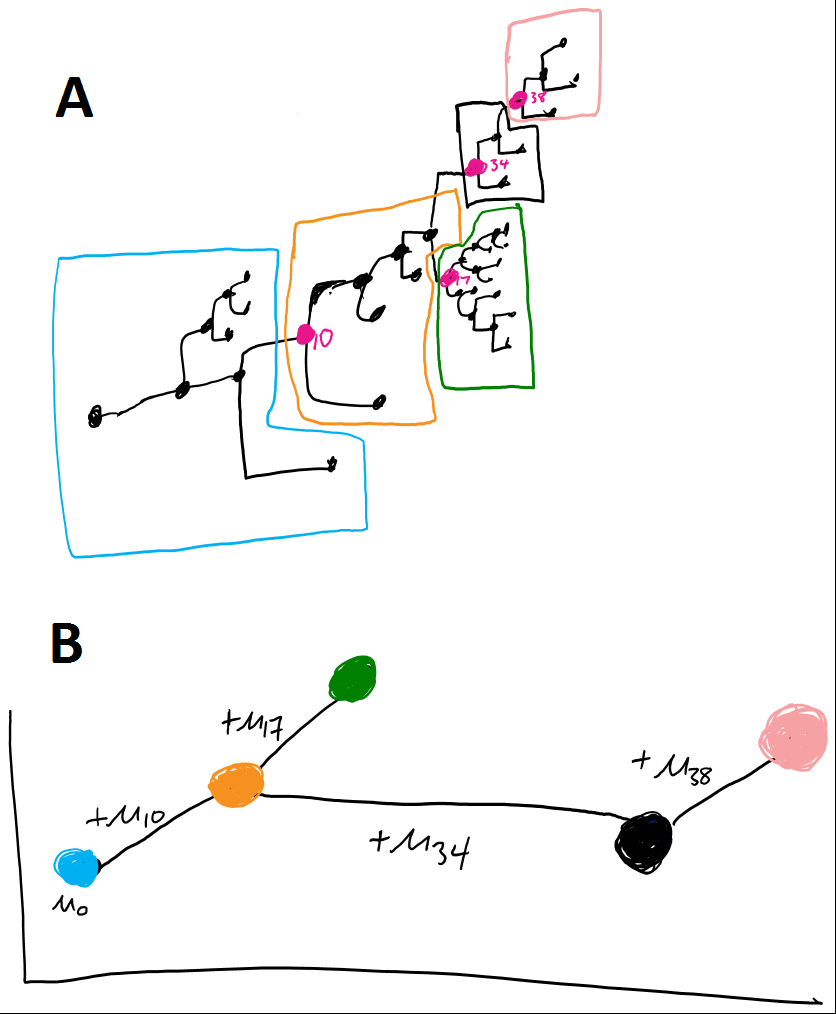
\includegraphics[width=0.5\textwidth]{figures/autoregressiveModel}
	\caption{\textbf{Phylogenetic Clustering and Autoregressive model.} 
(A) Each node on this phylogenetic tree $T$ is represented by a circle. 
Node 10, 17, 34, and 38 are active (purple; $I_{10}=I_{17}=I_{34}=I_{38}=1$) and each remaining node is inactive (black; $I_i=0$). 
These active nodes partition the viruses, which are the external nodes, into 5 clusters.
(B) Antigenic map of viruses are drawn using the set of $\mu_i$s that are associated with the $T$ and $I$ above. 
For example, the green and black clusters are branched off from the orange cluster. 
The blue cluster is the root cluster given an initial location $\mu_0$.
%for consistency, should be changed to N
	} 
	\label{autoregressiveModel} 
\end{figure}


%need to understand if ``autoregressive'' is the correct word.	
\subsubsection*{Overview}
Our method incorporates several statistical and computational techniques. 
First, to perform phylogenetic inference via sequence data, we used the software BEAST, after which a Maximum Clade Credibility (MCC) tree is obtained for antigenic clustering.
Second, to extract the most significant patterns from the antigenic data while simultaneously capturing uncertainties in the inference, we used the Bayesian MDS algorithm \cite{oh_bayesian_2001}.
Third, to focus on identifying branches that are associated with major antigenic changes, we inferred antigenic clusters using the Bayesian Stochastic Search Variable Selection (BSSVS) method on nodes in the inferred phylogeny, a technique previously used by the phylodynamic \cite{lemey_bayesian_2009, drummond_bayesian_2010} and more generally by the Bayesian community \cite{kuo_variable_1998, hugh_chipman_practical_2001}.
Fourth, to relate antigenic clustering with antigenic distance from one parental cluster to a child cluster, we applied an autoregressive model \cite{drummond_bayesian_2010}.
%that has recently been applied to phylogenetic inference.Figure~\ref{autoregressiveModel}A-B. 
Finally, to perform this Bayesian inference, we used the Markov chain Monte Carlo (MCMC) technique along with specialized proposals to sample from the posterior distribution. 







\subsubsection*{Antigenic Clustering using a Phylogeny}

In our model, antigenic clustering is fully parameterized by  a phylogeny and a vector of indicator variables.
%Given an inferred phylogeny $T$, we partition viruses into distinct antigenic clusters $T$ (Figure~\ref{autocorrelationModel}).
A phylogeny $T$ consists of N total nodes that include $n_v$ external nodes representing the set of viruses and $N-n_v$ internal nodes connecting the external nodes.
Associated with each node $i$ is a binary indicator variable $I_i \in \{0,1\}$. 
Here, we define a node $i$ as active if $I_i = 1$.
When node $i$ is active, this node and all its descending nodes are branched off into a new cluster from the parent node of $i$.
The root node is always active (i.e. $I_{N} = 1$) because it gives rise to the first cluster.
By pre-order traversing $T$ from the root node along with a configuration $I=(I_1, ..., I_N)=(i_1, ..., i_N)$, cluster labels are assigned to viruses (Figure~\ref{autoregressiveModel}).
%The algorithm for this tree traversal procedure is described in the Appendix. - necessary?


In phylodynamic literature, the Bayesian inference of the parameter $I$ is referred to as the Bayesian Stochastic Search Variable Selection procedure (BSSVS) \cite{lemey_bayesian_2009}.
This procedure has been applied in a setting to determine the subset of parameters in the phylodynamic transition matrix that are nontrivial. 
Here, our usage is similar to one used in the Bayesian random local clocks model implemented in BEAST \cite{drummond_bayesian_2010}.
In our work, the BSSVS is performed on the nodes in the phylogeny to identify the subset of nodes that branch off into new antigenic clusters. 
Each indicator $I_i$, for $i=1,..N-1$, has an equal prior probability to be active.
%note: , 

%DESCRIBE the variable selection as a complicated problem... (N)x(N-1)x(N-2)x.... possibilities!
%computationally impractical...


\subsubsection*{Autoregressive Model for Antigenic Locations of Viruses}

We connect phylogenetic clustering with antigenic trait by using an autoregressive model to assign antigenic locations to viruses. 
Our model assumes that all viruses in the same cluster share the same antigenic coordinate and viruses in different clusters have different antigenic coordinates.
This modeling decision is motivated by the evidence that only a small fraction of driver mutations contribute to substantial antigenic drift \cite{koel_substitutions_2013}, so our priority here is to parsimoniously model the most substantial antigenic changes.



While we are only interested in the antigenic location of the $n_v$ viruses corresponding to the external nodes $X=(X_1,..., X_{n_{v}})$, $X_i \in \mathbb{R}^{2}$, we first consider the augmented space $X' = (X_1, ...X_{n_v}, X_{ n_v +1},..., X_N)$ that consists of locations of both  external and internal ($X=(X_{n_v + 1},..., X_N)$) nodes.
Initially, we define
\begin{eqnarray}
 	X_{N} = \mu_N     ,
\end{eqnarray}
 where this last index $N$ corresponds to the internal root node and $\mu_N \in \mathbb{R}^{2}$ is a parameter representing the antigenic change from the origin, which in this case is the absolute antigenic location associated with the root node. 

We perform a pre-order traversal on the entire set of nodes in $T$  from the root node to assign antigenic locations of the remaining nodes by using an autoregressive model along with the vector $\mu = (\mu_1,...\mu_N)$, where $\mu_i = (\mu_{i1},  \mu_{i2}) \in \mathbb{R}^{2}$ represents the antigenic change from the parent node to the child node.
\begin{equation}
	X_i=  X_{p(i)} + \mu_i    I_i   		,
\end{equation}
for each of $i=1,... N$, where $p(i)$ denotes the parent of node $i$.
Thus, if $I_i=0$, node i inherits the identical location as that of its parent because the effect of $\mu_i$ is turned off, and if $I_i=1$, the location of node i has an offset of $\mu_i$ from its parent.
At the end of the tree traversal, the antigenic location of all viruses will be determined.
Algorithmically, the antigenic location assignment is done in conjunction with the previously described tree traversal procedure for assigning cluster labels.


%give historical annodote where this kind of model is used.
%Traditionally, this model has been extensively used in time series...econometric? financial data..?

This autoregressive model is appealing for a couple of reasons.
First, this model explicitly infers the change in antigenic distance $\mu_i$ from one cluster to the next.
Second, this model partitions viruses in a way that is related to the evolution process as specified by $T$.
This model naturally delineates the path of clusters transition, a feature that is also new to this clustering method.



% and $I$ is the identity matrix with 1 in the diagonal and 0 in the off-diagnoal cells. [Note. need another symbol. I is used.]



\subsubsection*{Bayesian Posterior Inference}

\begin{equation}
  p(Y, I, \mu ,  \beta | H, T, d) \propto  p(H| X(T, \mu, I), Y , \mdssd^2) p(Y|  \beta, d) p(I) p(\mu) p(\beta)
\end{equation}

Our full model consists of several components.
The first component $p(H|X(T, \mu, I),Y )$ specifies the antigenic likelihood of the observed antigenic data $H$.
The antigenic likelihood is based on the MDS framework, in which $H$ is explained by the coordinates of the viruses $X=(X_1, ..., X_{n_v} )$ and sera $Y = (Y_1, ..., Y_{n_{s}} )$  in the two dimensional antigenic map.
As previously described, $X$ is determined by $T$, $\mu$, and $I$.
The parameter $\mdssd^2$ specifies the variance around the expected log$_2$ titer value for an observed measurement, which is described in detail in the Method section.
We define the tuning parameter for antigenic clustering as the precision term in the antigenic likelihood
\begin{equation}
  \kappa = \frac{1}{\mdssd^2}.
\end{equation}
A higher $\kappa$ sets the model to tolerate less noise around the expected log$_2$ titers.
Thus, increasing the value of $\kappa$ encourages the antigenic clustering method to identify more clusters.
The antigenic likelihood is further discussed in the Method section.
The second component $p(Y|  \beta , d)$ defines the prior for sera locations $Y$, conditional on the dates of sera ($d$), the drift parameter $\beta$, and the fixed serum variance $\sigma^2_s$ of 1. 
The next components $p(I)$ , $p(\mu)$, and $p(\beta)$ define the prior for $I$, $\mu$, and $\beta$, respectively.
We assume an equal probability $p$ for each $p(I_i = 1)$.
We assume an independent and identically distributed normal prior for $\mu_i$, $i=1,...N$ for each dimension $j \in {1,2}$.
\begin{equation}
   \mu_{ij}  \sim N( 0 , \sigma^2_\mu)			,
\end{equation}
We assume a noninformative inverse gamma(0.0001,0.0001) for $\beta$.
$\sigma^2_\mu$ is given a value of 2.5, so that the average absolute displacement would be $\sim$2 units, which is the average value of change in the antigenic map during antigenic transitions for A/H3N2 \cite{jong_antigenic_2007}.
Roughly speaking, this prior thus encourages us to identify transitions that is around 2 units, corresponding to a 4-fold reduction in fold change from the maximum titer.
% I remembered you said there a unit of 2 is related to WHO? source? what's the precise argument?
%(I actually parameterized as precision) - precision = 0.4
We describe the remaining components, details of the Bayesian Antigenic Cartography, and the MCMC procedure in the Method section.



\newpage







\newpage

%%% RESULTS %%%
\section*{Results}

% I guess I need your assistance in abstracting knowledges acquired from this study to a higher level to understand what are the more significant messages

\subsection*{Analysis of the A/H3N2 and A/H1N1 Datasets}


\subsubsection*{A/H3N2}
%Substantially more antigenic clusters were inferred in A/H3N2 (Figure \ref{H3N2tree} and \ref{H3N2heatmap}) than in A/H1N1. 
The antigenic phenotypes of A/H3N2 evolves substantially quicker (Figure \ref{H3N2tree} and \ref{H3N2heatmap}) than A/H1N1 during a comparable timeframe.  %need a  year maybe..
At the default $\kappa=0.05$, our method inferred 15[edit] clusters with at least 5 observed viruses.  
At the higher $\kappa=0.15$, our method inferred $\sim$20[edit]. 
%I think I omitted ementioning $\kappa=0.1$. 
%I think I might not have mentioned comparison to $\kappa=0.15$ enough. not sure what to say.
Similar to the results from A/H1N1, the higher number of clusters at $\kappa=0.15$ was a consequence of subdividing within the inferred clusters at $\kappa=0.05$, which is a desired property when changing $\kappa$.
The consistent antigenic boundaries at $\kappa=0.05$ were maintained (Figure \ref{H3N2heatmap}). 


\begin{figure}[h]
	\centering		
	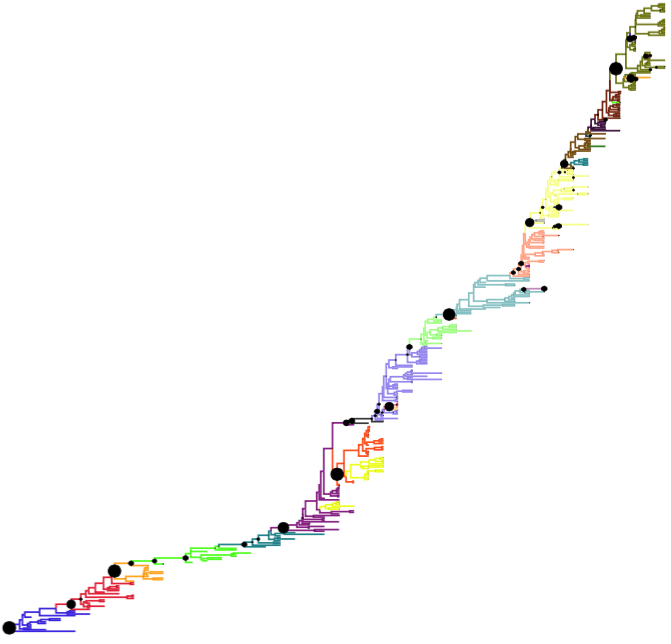
\includegraphics[width=1\textwidth]{figures/custom/H3N2MCC}
	\caption{\textbf{}
	 		} 
	\label{H3N2tree} 
\end{figure}



\begin{figure}[h]
	\centering		
	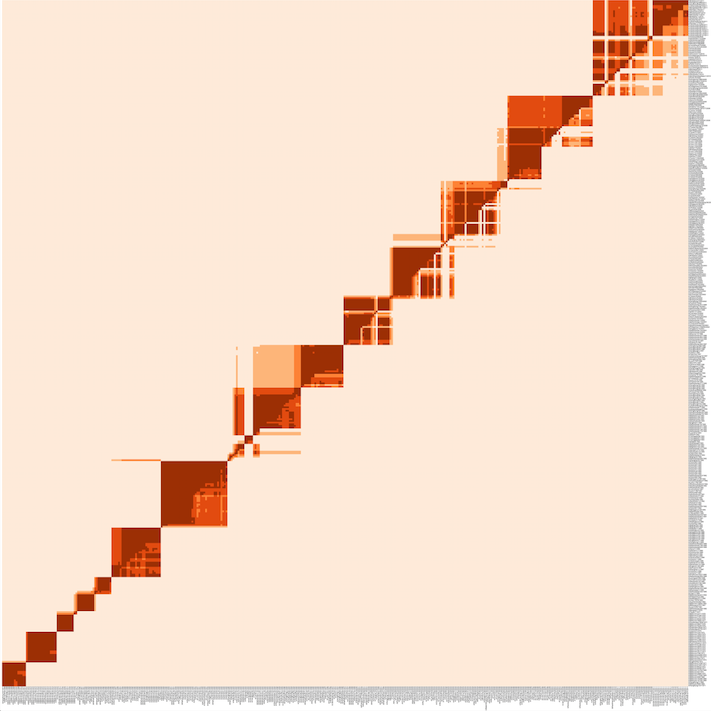
\includegraphics[width=1\textwidth]{figures/custom/H3N2Heatmap}
	\caption{\textbf{A/H3N2}
	 		} 
	\label{H3N2heatmap} 
\end{figure}



The clustering method at the default $\kappa=0.05$ recovered with high confidence almost all the  antigenic clusters inferred by Smith et al. \cite{smith_mapping_2004}. 
Concordant to Smith's results, the HK68, EN72, BK79, VIC75, SI87, BE89, BE92, WU95, SY97, FU02 virus strains were classified to belong to distinct antigenic phenotypes. %give precise strain names?
For the TX77 strain identified by Smith et al. \cite{smith_mapping_2004}, our clustering method also detected some evidence that it was antigenically different from its neighboring clusters but without much certainty.
This is likely due to small sample size, with only TX77 and potentially A/Bilthoven/2271/1976 showing the most evidence of co-clustering (Figure \ref{TX77heatmap}). %co-clustering = right word?
Instead, the TX77 strain shows evidence that it is both associated with the earlier (EN72) and later (BK79) clusters .
Complementary to Smith's results, our result also inferred that each EN72, VIC75, (TX77), BK79, BE89, BE92, and SY97 strain was either on the branch leading to antigenic transition or was very close to it, while the HK68, SI87, WU95,FU02 were in the middle of the cluster. 


%probably a supplementary figure.
\begin{figure}[h]
	\centering		
	
\includegraphics[width=0.3\textwidth]{figures/custom/H3N2heatmapTX77}
	\caption{\textbf{The TX77 sub-heatmap.} A/Bilthoven/2271/1976 and A/Texas/1/1977 are in the middle cluster - upper triangle = $\kappa=0.05$ and higher triangle=$\kappa=0.15$
	 		} 
	\label{TX77heatmap}  
\end{figure}



With more recent data, our analysis inferred the emergence of three major antigenic phenotypes of nontrivial size ($>5$ viruses) since the end point of Smith's analysis \cite{smith_mapping_2004}.  
These clusters were highly plausible, because they were associated with strains used in historic vaccine updates during the 2005-2006 (CA04), 2008-2009 (BR07), and 2010-2011 (PE09) flu seasons \cite{WHO VACCINE REPORT}. 
%http://en.wikipedia.org/wiki/Influenza_A_virus_subtype_H3N2
%full name?
Interestingly, PE09 was updated to VIC09 after 1 year during 2011-2012, and our results also provided evidence that VIC09 was antigenically different from PE09, even though this VIC09 cluster only had two strains.
During this period, the only other notable vaccine strain used was A/Wisconsin/67/2005 for the 2006-2007 flu season.
Our results suggested some evidence but not with certainty (~$\sim$ 25\% on one internal node and $\sim$ 13\% on the next internal node leading to the A/Wisconsin/67/2005 strain) that this strain is antigenically different from the CA04 cluster.

Our results also inferred other antigenically distinct clusters previously not identified. 
This includes two clusters in the trunk, represented by the A/Wellington/4/1985 (green) and the Netherlands 1993 [a fullname wanted] strains (Figure \ref{H3N2tree}), and a few smaller clusters, represented by A/Yamagata/61/1993, A/Sofia/141/2003, A/Osaka/56/2004,  A/Singapore/2004, and A/Victoria/208/2009. 
The A/Singapore/36/2004 singleton cluster has probability 45\% of being antigenically distinct, but it may be a false positive because its neighbor strain A/Singapore37/2004  shows no evidence to be antigenically distinct from their common ancestral cluster. 
On the other hand, the A/Yamagata/61/1993 cluster, associated with a probability of 69\% being antigenically distinct, makes a partition leading to 5 observed virus strains.
This amount of aggregated evidence suggests that this partition may be a true antigenic transition that was not previously recognized due to lack of progenies. 




Our inference infers the location of antigenic transitions (Figure \ref{H3N2tree} and \ref{H3N2heatmap}). 
9 inferred antigenic transition were each attributed to a single branch with probability $>50\%$. In each of the 5 other transitions, the result shows uncertainty in inferring a branch that leads to an antigenic transition. 
This highlights that a probabilistic clustering method can quantify the statistical uncertainty. %Uncertainty may arise because of "antigenic continuum", absence of data that could resolve this discrepancy, or random noise. - discussion item?




Antigenic cartography of A/H3N2 reveals several interesting characteristics (Figure \ref{H3N2Euclid}). 
Antigenic distance moves relatively linear with time.  
This result is consistent with previous analyses \cite{smith_mapping_2004, bedford_integrating_2014}, but might partially be a consequence of the diffusion prior, which apriori scales the first dimension of the serum location linearly by $\beta$. 
Nevertheless, the BE89 cluster diverges substantially into the second dimension, similar to the previous results of antigenic cartography \cite{smith_mapping_2004, bedford_integrating_2014}. 
We detected divergence into the second dimension with the A/Yamagata/61/1993 cluster and in some very small clusters. 
Among nodes with substantial evidence of antigenic transitions ($\hat{p_i} > 0.5$), the average change in antigenic distance is $\sim$3.5 [edit]. 
 We observed the largest antigenic change from BR07 to PE09 ($\sim$7.x unit), from WU95 to SY97 ($\sim$5.x unit), and from EN72 to VIC75 ($\sim$6.x unit) (Figure \ref{H3N2muplot} and \ref{H3N2ediston}).
[what else is interesting?]




\begin{figure}[h]
	\centering		
	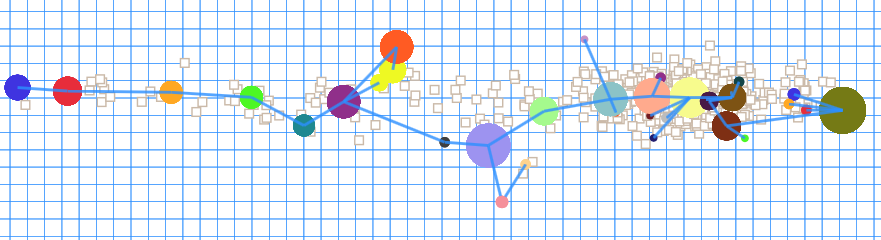
\includegraphics[width=1\textwidth]{figures/custom/H3N2Euclid}
	\caption{\textbf{A/H3N2}
	 		} 
	\label{H3N2Euclid} 
\end{figure}




\begin{figure}[h]
	\centering		
	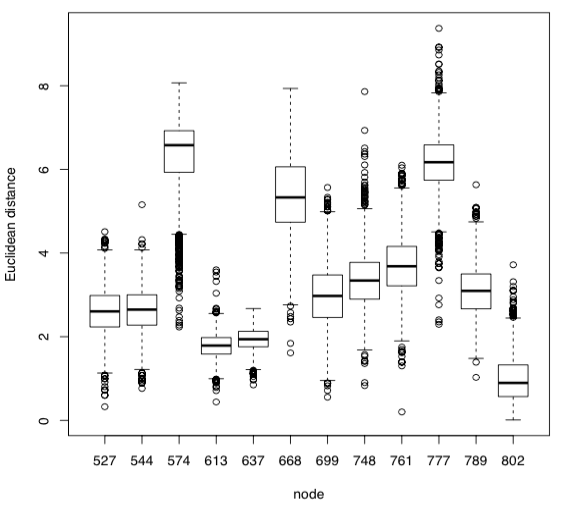
\includegraphics[width=0.7\textwidth]{figures/custom/H3N2Muboxplot}
	\caption{\textbf{Boxplot of the Euclidean distance of distribution of $\mu_i$, conditional on $I_i = 1$,  from the parent clusters for the A/H1N1 analysis with $\kappa=0.05$}
	 		} 
	\label{H3N2muplot} 
\end{figure}



\begin{figure}[h]
	\centering		
	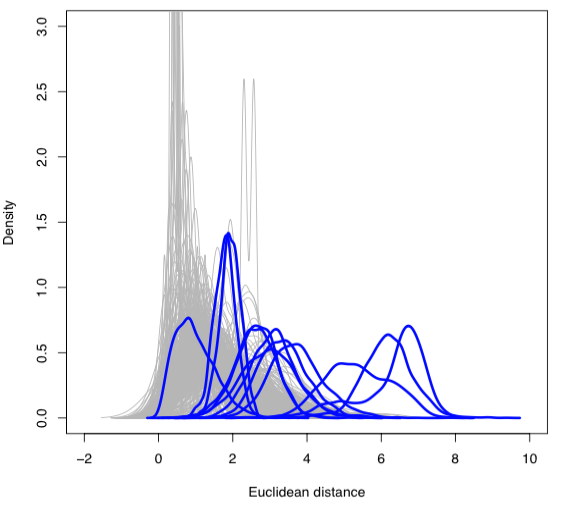
\includegraphics[width=0.7\textwidth]{figures/custom/H3N2EDistOn}
	\caption{\textbf{Histogram of the Euclidean distance of $\mu$ from the parent clusters for the A/H3N2 analysis with $\kappa=0.05$.}
	 		} 
	\label{H3N2ediston} 
\end{figure}


\subsubsection*{A/H1N1}
In A/H1N1, six major antigenic clusters were inferred between the 1977 and 2009 virus strains (Figure \ref{H1N1-tree}). 
Under the default  $\kappa=0.1$, the method was able to assign viruses to very distinct antigenic blocks  (Figure \ref{H1N1-heatmap}). 
Within-block structure suggests mild evidence that the viruses from 2006 to 2009 (light green cluster - Figure \ref{H1N1-tree}) could be further divided into two or three sub-clusters. 
At $\kappa=0.3$, detection of more antigenic transitions were encouraged. 
The overall clustering pattern looks very similar to that of the default $\kappa$ (lower triangle -  Figure \ref{H1N1-heatmap}). 
Nevertheless, at this higher $\kappa$, the method identified some other viruses, such as the single A/Iceland/8064/2009 strain, to be antigenically different from their neighbor viruses in the phylogeny. 


\begin{figure}[h]
	\centering		
	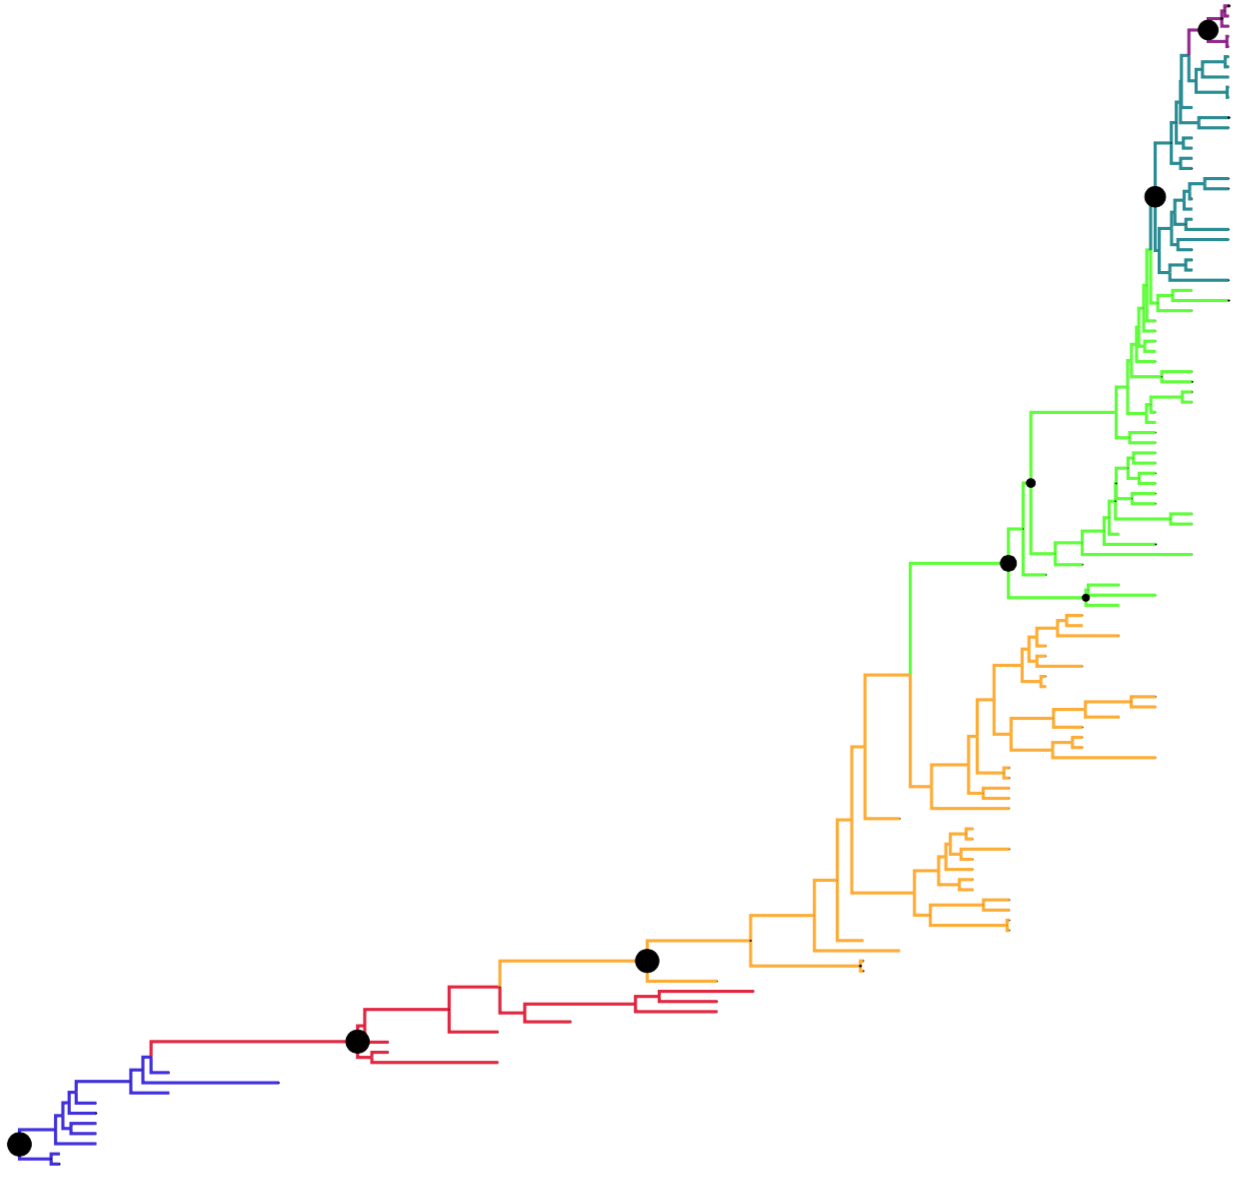
\includegraphics[width=1\textwidth]{figures/custom/H1N1MCC}
	\caption{\textbf{Inferred antigenic clusters on the A/H1N1 MCC phylogeny.}
 The color of the clusters corresponds to the one sample of clustering that gives the highest posterior density. The area of each node annotates the probability that a node is on. The root node has probability = 1. In this analysis, the default $\kappa$  at 0.1 is used.
	 		} 
	\label{H1N1-tree} 
\end{figure}



\begin{figure}[h]
	\centering		
	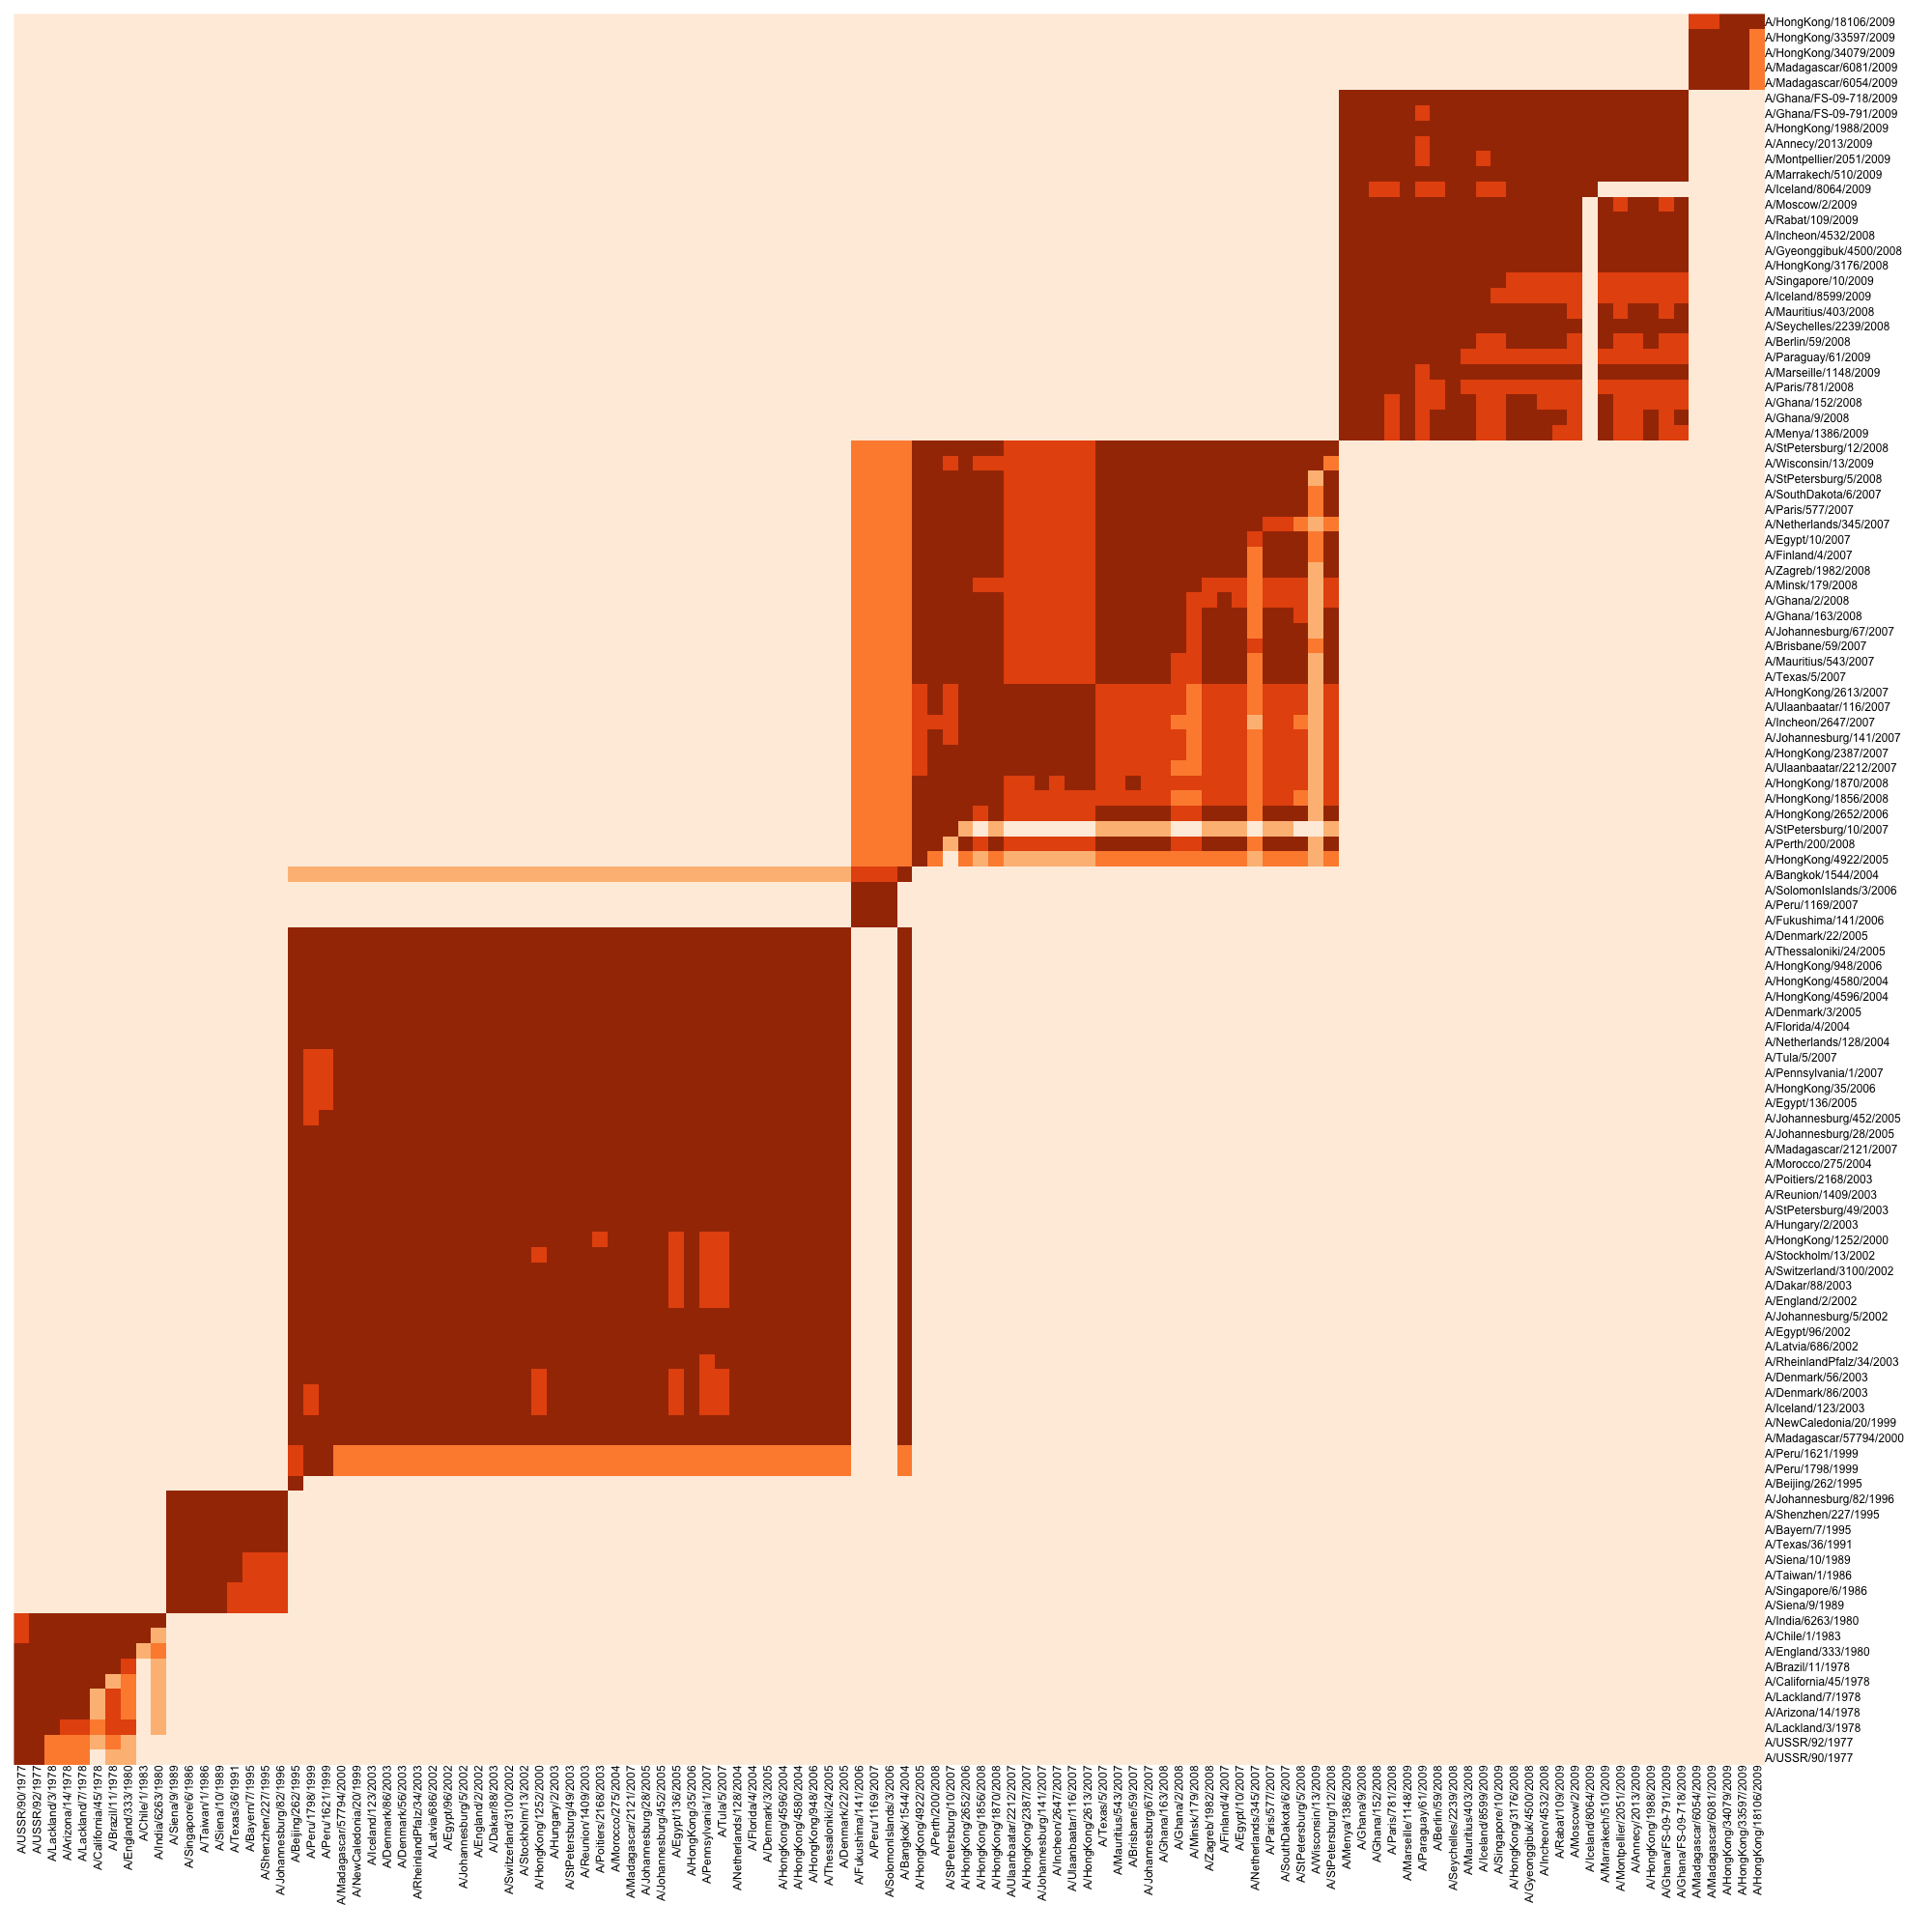
\includegraphics[width=1\textwidth]{figures/custom/H1N1mds01vs03ordered}
	\caption{\textbf{Heatmap plot summarizing probabilistic clustering in A/H1N1 viruses at $\kappa$ of 0.1 (upper triangle - default condition) and 0.3 (lower triangle).}
Each point represents the estimated probability  in which the virus in row $i$ and the virus in column $j$ belong to the same antigenic cluster, with darker color representing higher probability.  
The viruses were ordered by the MCC phylogeny in Figure X.
	 		} 
	\label{H1N1-heatmap} 
\end{figure}


%The number of years until antigenic transition is not constant.  
%next sentence, # years...
%It is possible that it is due to differential sample size across years, which affects the chance of cluster detection. 
%In later years where sampling becomes much denser, the power to detect different variants may become higher.

%I don't think my interpretion is good enough, but how can we improve it?
%Also, I don't know if I should make parallel comparison for A/H3N2. If so, do you want to try?
The antigenic map (Figure \ref{H1N1antigenicMap}) reveals three characteristics.
First, the antigenic distance jumps by an average of 4 unit during antigenic transitions. 
Second, nodes with significant evidence for antigenic cluster transition ($p_i > 0.5$) tend to have higher posterior mean change in antigenic distance than the other nodes (Figure \ref{H1N1Muboxplot}).
%not sure if the third point is good..
%any more observations from the antigenic map?
Third, the later antigenic transitions jumped less in antigenic distance than the early antigenic transitions (Figure \ref{H1N1MuEDistOn}). 
To distinguish whether this result is an artifact induced by the specification of the Diffusion prior, which models the mean first dimension of the serum location by linearly scaling the serum offset date by the serum drift parameter ($\beta$), we divided the Euclidean distance of the antigenic change by the number of years before antigenic transition. [probably need a table and refer to some numbers]
Surprisingly, we observed that the average antigenic movement per year actually became higher for later transitions. 
Thus, this may be an artifact induced by uneven sampling.


%I just did this data collection calculation by hand
%virus strain  [adjust by the emerence year of the new antigenic transition]  (# years until antigenic transition)	#Euclidean distance/years
%77-83  (6)	5/6=0.8333 
%86-96   [95] (9)	6/9=0.6667
%95-2007 [2006] (11)	3/11=0.25
%2006-2009 [2008] (2)	3/2=1.5
%2008-2009 (1 )	2.5/1=2.5
%2009 (0)





\begin{figure}[h]
	\centering		
	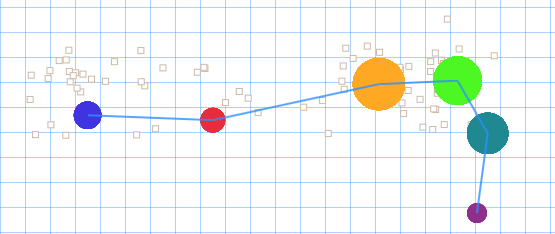
\includegraphics[width=1\textwidth]{figures/custom/H1N1Euclid}
	\caption{\textbf{Maximum a posteriori (MAP) estimate of Antigenic map of A/H1N1.} %MAP = sample at the highest posterior value?
 Virus clusters are drawn in circles, with the area of the circle scaled by the cluster size. Sera are drawn in squares.
	 		} 
	\label{H1N1antigenicMap} 
\end{figure}






%maybe this belongs to the Supplementary materials?
\begin{figure}[h]
	\centering		
	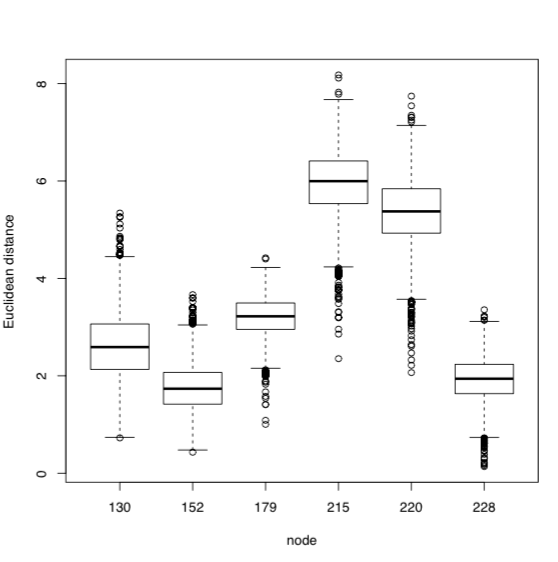
\includegraphics[width=0.7\textwidth]{figures/custom/H1N1Muboxplot}
	\caption{\textbf{}
Boxplot of the Euclidean distance of distribution of $\mu_i$, conditional on $I_i = 1$,  from the parent clusters for the A/H1N1 analysis with $\kappa=0.1$
	 		} 
	\label{H1N1Muboxplot} 
\end{figure}



\begin{figure}[h]
	\centering		
	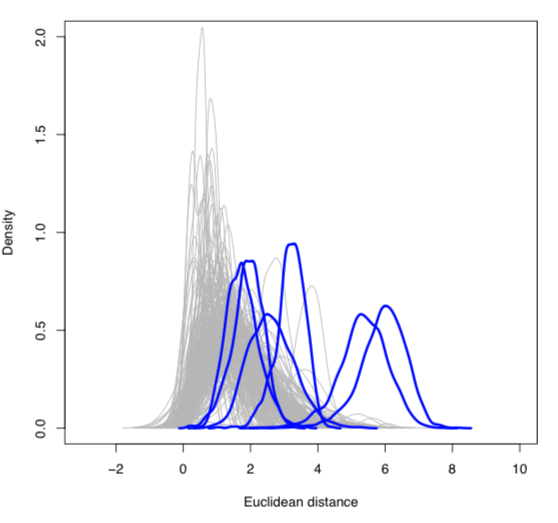
\includegraphics[width=0.7\textwidth]{figures/custom/H1N1EDistOn}
	\caption{\textbf{}
Histogram of the Euclidean distance of $\mu$ from the parent clusters for the A/H1N1 analysis with $\kappa=0.1$.
	 		} 
	\label{H1N1MuEDistOn} 
\end{figure}




\subsubsection*{Sensitivity Analysis}

Diagnostics for MCMC convergence suggest that the MCMC mixing are adequate in both A/H1N1 and A/H3N2 analyses. 
First, comparing among replicates, the estimates of $p_i$ are almost identical (supplemental Table SX-Y). 
The scatterplot of the distribution of these estimates in each pair of replicates shows very high concordance, with $R^2 > 0.9x$  for A/H1N1 (Figure SX-Y) for each level of $\kappa$ considered. 
We expected that the A/H3N2 analysis would have more difficulty with MCMC mixing than the A/H1N1 analysis because the complexity of the MCMC inference is higher due to substantially more observations and more antigenic clusters. 
Nevertheless, MCMC mixing still appears to be adequate ($R^2 > 0.9x$) (Figure SX-Y). 
Second, the Gelman-Rubin statistic further suggests adequate mixing in each $p_i$, with values below 1.2  suggesting convergence \cite{Yang_evolutionbook}. 
Third, the Effective Sample Size statistic suggests that the effective number of independent MCMC samples ($>1000$[edit]) and diagnostic plots obtained from Tracer (Figure SX-Y) suggests that other parameters also mixed adequately.

The clustering results are consistent across the use of different trees sampled from the original MCMC phylogenetic inference. In each comparison, the heatmap comparing probabilistic clustering from the MCC tree and a sampled tree (Figure S X-Y  for A/H1N1 and X- Y for A/H3N2) shows that the clustering patterns are highly similar. 
For instance, viruses that are inferred to have a high probability of co-clustering in one tree also has a high probability of co-clustering in other trees, and the distinct block structures are preserved. 
Variation from results among tree samples does exist but are minor (Figure S X - Y). 
Hence, this sensitivity analysis further verifies that the use of a single MCC tree is reasonable.


\subsection*{Simulations}
Results from computer simulation suggest that our clustering method effectively infers true antigenic transitions (Figure \ref{ROCSimulation}). 
Under the default $\kappa=0.1$, at the 50\% data completion, our method detects an average of 14.x of the 15 simulated transitions (sensitivity= 9x\%) while controlling the average number of false positives to $<1$. 
As a true positive is defined stringently by the exact matching of a node that leads to an antigenic transition, this result comes as a welcome surprise because before the simulation it is not understood whether the method can detect the exact node or can only detect up to a proximity of where the true transition node is.
Interestingly, sensitivity remains almost as high at lower data completion rates (average true positives = $\sim$14 and $\sim$14 for data completion at 20\% and 10\%, respectively) with similarly low average false positives. 
However, the average number of true positives decreases dramatically to $\sim$8 when the data completion decreases to 5\%. 



%%% Result Figure %%%
\begin{figure}[h]
	\centering		
	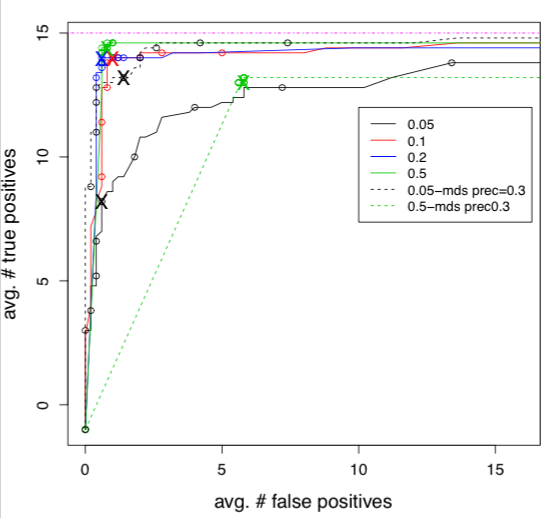
\includegraphics[width=0.7\textwidth]{figures/custom/ROC-simulation}
	\caption{\textbf{The impact of varying the data completion rates on the performance of inferring antigenic clusters is summarized by the Receiver Operating Characteristic curves.} 
 The results were averaged across 5 replicates.	
 Dots are drawn from the right to the left at a decreasing threshold of p=1,0.9, 0.8, ...,0.1. 
 The symbol X defines the threshold at p=0.5. 
The purple dotted horizontal line defines the total number of true simulated transition events. 
Here, true positives and false positives are summarized as absolute numbers instead of percentages because the former scale facilitates interpretation of the results and gives a more appropriate perspective of the underlying simulation condition.
	 		} 
	
	\label{ROCSimulation} 
\end{figure}






Setting $\kappa$ to a higher value is beneficial when data completion is low but not when it is high (Figure \ref{ROCSimulation}). 
By increasing $\kappa$ from 0.1 to 0.3 to encourage detection, the number of true positives jumps substantially from $\sim8$ to $\sim$13.5 even at the 5\% data completion. 
Setting a higher $\kappa$ also increases the average number of false positives from $\sim0.5$ to $\sim$1.5. 
The true to false positive trade-off suggests that the use of a higher $\kappa$ is justified. 
However, setting a higher $\kappa$ is not preferable when the data completion rate is high, because this would also detect more noises. 
At 50\% data completion, setting $\kappa$ from 0.1 to 0.3 not only reduces the number of true positives from $\sim$14.5 to $\sim$13 but also increases the number of false positives from $<1$ to $\sim$ 5. 
One hypothesis that explains this decrease in performance is that the clustering method tends to over-classify viruses (Figure \ref{QUALITATIVE_OBSERVATION}).
This may be due to  spurious association from non-random observed measurement noises occurring by chance even though our simulation generates completely random noises. 
In this case, the use of a lower $\kappa$ effectively guards against false positives.





\newpage

\section*{Discussion}

% maybe worth bringing out the main scientific results? If so, what are they?
%how do I organize the first paragraph? right content put? or what to say instead
We developed an antigenic clustering method that extends the antigenic cartography in the Bayesian framework to integrate information from a phylogeny. 
%This method is intuitive because antigenic transitions occur as viruses evolve. 
This probabilistic-based method captures the uncertainty associated with the inference, enabling investigators to understand the level of confidence associated with each inferred antigenic transition. 
We successfully applied this method to real analyses and obtained meaningful results.
In addition, we demonstrated that the BSSVS framework, since its introduction to phylodynamics \cite{lemey_bayesian_2009, drummond_bayesian_2010}, can also be applied to cluster virus strains on a phylogeny by data from a high dimensional trait.  % is it okay to  keep it here? or does this sentence belong to somewhere else?
%if so what else should I say here?

The use of phylogeny complements/offers advantages over existing methods. 
First, by leveraging a phylogeny, our model explicitly relates the emergence of antigenic phenotypes with genetic evolution, which enables the estimation of some important parameters of interest. 
In particular, we can infer the probability of antigenic transition at each branch corresponding to the node, path of antigenic transition, and antigenic changes associated with each cluster transition. 
Second, as phylogeny itself is clustering, this information provides tremendous value to antigenic clustering when antigenic data is added. 
Third, via BSSVS on the nodes of phylogeny, our task of clustering is greatly simplified. 
Fourth, our model naturally minimizes misclassification of viruses because it prevents any two viruses that are close together in the antigenic map to be in the same cluster when there is an active internal node between the two viruses in the phylogeny.

This method inferred highly plausible antigenic clusters for A/H1N1 and A/H3N2. 
For  A/H3N2, we validated that our results agreed very well with the previously characterization from 1968 to 2004 \cite{smith_mapping_2004} and inferred new antigenic clusters up to 2010. 
Our results suggested that some branches are associated with major antigenic changes, which agrees with an experimental validation that only some important substitutions causes recent antigenic evolution of HA \cite{koel_substitutions_2013}. 
Some of these branches were inferred with high confidence. 


In A/H3N2, the use of a higher $\kappa$ reveals antigenic substructure. 
The use of a higher $\kappa$ tends to break some cluster of viruses inferred by a lower $\kappa$ into subgroups. 
Some of these groups may even consist of just one or a few viruses. 
Perhaps this result gives some evidence of "antigenic continuum", that more virus strains than we previously classified may be (slightly) antigenically different from their parent strains. 
This viewpoint complements, rather than contradicts a previous viewpoint that some substitutions significantly affect antigenic distances \cite{koel_substitutions_2013} because the focus of that work is on identifying substitutions from 10 clusters instead of performing an exhaustive characterization on the effect of every mutation. 
It is also possible that some antigenically distinct phenotypes emerged, but those viruses did not propagate to form large clusters.
Alternatively, very small clusters, especially those inferred at a larger $\kappa=0.3$, might be due to false positives that were detected because of measurement noises or systematic batch effects.
Regardless, the results that the original boundaries for antigenic transitions at lower $\kappa$ continues to be the same boundaries at higher $\kappa$ consistently suggests that major antigenic transitions do exist. 
When the priority is to only identify these major transitions, e.g., for antigenic surveillance, the use of a lower $\kappa$ is justified.  
%I think this point is interesting [not sure if it is completely novel], but do you think the evidence is solid enough and the finding is significant such that this point should be discussed in the abstract and somewhere earlier as well?


To achieve adequate MCMC mixing, we developed proposal distributions specific to this model. 
While the antigenic clustering model appears to be just an extension of the Bayesian multidimensional scaling \cite{bedford_integrating_2014}, the combination of BSSVS on phylogeny with a trait infers by multidimensional scaling via autoregressive model presents nontrivial challenges to proposing MCMC transitions that are effective. 
Our research experimented with different proposal distributions to understand the underlying factors that allows or prevent effective proposals. 
In this case, we discovered that effective MCMC mixing may require (1) joint moves on some key parameters that are associated with locations of viruses or sera on the antigenic map and (2) transitions that do not dramatically impact the relationship on the map.


This work leads to several potential future extensions. 
First, the current model assumes that each node has an equal prior probability of antigenic transition. 
An extension may use the inferred branch lengths to adjust this prior probability, allowing longer branches to have higher apriori probability to be active.
Second, the model currently conditions on one single tree. 
Extension of this work may consider the use of multiple phylogenetic tree samples, a simultaneous inference of antigenic and phylogenetic inference via sequence and antigenic data, or  an error model on clustering for misplacement of viruses on an inferred phylogeny, even though our results suggested that the use of different trees made little impact to the inference. 
Third, this work may have implication to vaccine strain selection. 
This systematic and integrative approach may help with timely antigenic classification. 
Future evaluation is needed to evaluate its power in inferring emerging antigenic phenotypes. 
Fourth, building onto this work, it may be possible to develop an effective genotype to phenotype mapping strategy (e.g. with ancestral state reconstruction) to identify mutations associated with antigenic transitions. 
Investigation and development of potential approaches should warrant effort that is beyond the focus and scope of this work.



%Our method has broad applicability.



\newpage




%%% MATERIALS AND METHODS %%%
\section*{Methods}


\subsection*{Antigenic Cartography via Bayesian Multidimensional Scaling}



\subsubsection*{Antigenic Likelihood }


The antigenic data consists of a matrix of HI titer measurements from $n_v$ viruses across $k$ sera.  
A HI titer ($H_{ij}$) measures the strength of cross-reactivity between virus $i$ and serum $j$, where $i=1, ...,  n_v$ and $j=1,...,k$, with high value suggesting high reactivity. 
The HI titers are usually obtained by serial dilutions, e.g. 40, 80, 160, etc, are commonly summarized as fold changes. These measurements are ordinarily analyzed in the scale corresponding to fold change by transforming the values by log$_2$ \cite{smith_mapping_2004, bedford_integrating_2014}, so that every unit difference suggests a change of titer by 2-fold. 
These HI titers can be thought of as a set of distances in a sparse $n_v$ by $k$ matrix, and with missing values because often the reactivity of a serum $j$ is not measured against the full set of viruses.
	%it's an incomplete matrix
	
Antigenic Cartography was proposed \cite{smith_mapping_2004} to condensely extract and visualize the main pattern from this matrix of distances. 
Antigenic Cartography is based on the multidimensional scaling algorithm to summarize this distance matrix into lower dimension by representing each virus and each serum by a 2-dimensional coordinate. 

Our method applies the Antigenic Cartography in the Bayesian framework \cite{bedford_integrating_2014}. 
The antigenic likelihood represents the likelihood of the observed HI titers. 
Each $H_{ij}$ is explained by the antigenic location of virus $i$ ($x_i$) and serum $j$ ($y_j$). 
Given $x_i$ and $y_j$, each measurement is assumed to be independent of each other. 
Thus, the antigenic likelihood is composed of multiplying the likelihood of all individual measurements.
%$x_i$ and $y_j$ is the realized value of the variable $X_i$ and $Y_j$, respectively. 

\begin{equation}
 p(H|X, Y, \mdssd^2) = \prod_{(i,j) \in \cal I} f(H_{ij} |  X_i  = x_i, Y_i = y_i,\mdssd^2) 
\end{equation}

Recall that the innovation in our model is that the virus locations are now determined by the antigenic change parameter $\mu$, node indicators $I$, and phylogeny $T$ using the procedure described in the New Approaches. 
For brevity, this function was omitted from the $X$ part in the equation above.

Let $s_j$ denote the serum potency, estimated by calculating the maximum log$_2$ titer of serum $j$ across the vector of observed log$_2$ titers from viruses that react with serum $j$.
\begin{equation}
	\se_j = \max ( H_{1j},\ldots,H_{\vn j} )
\end{equation}

We model the expected value of $H_{ij}$ as the departure from $\se_j$. Define

\begin{equation}
	\delta_{ij} =  || \virus_i - \serum_j ||_2,
\end{equation}
where $|| \cdot ||_2$ is an $L_2$ norm (Euclidean distance) between $x_i$ and $y_j$,

we then model $H_{ij}$ by the normal distribution with mean and variance given by 
\begin{equation} \label{hij}
	H_{ij} \sim \normal( \se_j - \delta_{ij}, \, \mdssd^2 ).
\end{equation}


 In reality, the titers are often left or interval censored. For instance, $<40$ suggests that the titer is a value between 0 and 40. To model these censored titers, the likelihood of observing a left censored observation is 

\begin{equation} 
	\threshold(H_{ij}) = \Phi \left( \frac{ H_{ij} + \delta_{ij} - \se_j }{ \mdssd } \right),
\end{equation}
where $\Phi(\cdot)$ represents the standard normal cumulative distribution function (CDF).

For an interval censored observation,
\begin{equation} 
	\interval(H_{ij}) = \Phi \left( \frac{ H_{ij} + \delta_{ij} - \se_j + 1 }{ \mdssd } \right) - \Phi \left( \frac{ H_{ij} + \delta_{ij} - \se_j }{\mdssd} \right).
\end{equation}



We use the Diffusion model for the prior antigenic locations of sera as previously described \cite{bedford_integrating_2014}. 
\begin{eqnarray}
	y_{j1} | d_j \sim N ( \beta d_j, \sigma^2_s )  \\
	y_{j2}  \sim N(0, \sigma^2_s)
\end{eqnarray}
where $d_j$ is the offset date calculated by subtracting the date of serum $j$ from the date of the earliest sampled virus or serum. 
As a consequence of this prior, the first dimension of the antigenic location of sera are spread out linearly by the dates of sera. 
$\sigma^2_s$ is set to a reasonable value of 1 that just controls how much we allow a serum to diverge from the prior antigenic location.
%\sigma^2_s is a nussiance parameter... I think any reasonable value would work... viruses will just get placed accordingly.
%Trevor, we agreed that 1 is a reasonable value. Do you have a better justification?

%Make sure to write in this information somewhere.
%mds precision set at.. default = 0.05
%serum drift ~ inversegamma(0.0001,0.0001)
%muMean=0
%muPrec=0.4
%serumPrec = 1  -
%probActiveNode ~Uniform[0,1]




%This property is desirable because virus evolves over time.  ?? better justification?



\subsubsection*{Posterior Sampling via Markov chain Monte Carlo}

To perform Bayesian inference on the parameters of interest, we resort to the use of the Markov chain Monte Carlo (MCMC) technique \cite{hastings_monte_1970, metropolis_equation_1953}.
The MCMC algorithm generates random samples that collectively approximate the posterior distribution.
In each MCMC iteration, a new state for a parameter is proposed from using a proposal distribution that conditions on the states of potentially multiple parameters obtained from a previous iteration.
%Equation
After drawing this new state, the MCMC calculates a number called the acceptance ratio.
Loosely speaking, the acceptance ratio is a device that enables the procedure to correct the sampling scheme so that at the end the samples approximate the desired distribution, even though the proposal distribution may be arbitrary.
The new state is accepted if the acceptance probability is larger than a random number drawn from the uniform(0,1) distribution; otherwise, the old state is used as the new state for this current iteration.
This procedure is repeated until a desired large number of iterations is obtained.


Via the Ergodic Theorem, the MCMC procedure generates a chain that converges to the posterior distribution \cite{hastings_monte_1970}. %is this the appropriate citation?
The use of sensible proposals could substantially improve the speed of convergence.
To this end, we studied a variety of proposals and retained the best proposal distributions that facilitate MCMC mixing.

%maybe i should avoid using the term transition kernel?
% proposal distribution vs. transition kernelß

\subsubsection*{MCMC Proposals}
%to evaluate, understand, and optimize the mixing behavior. 



The key to making efficient proposals on $\mu$ and $I$ is to devise proposals that make only slight change to the antigenic map.
The presence of the antigenic likelihood presents an interesting complication of efficiently exploring the posterior distribution via MCMC.
When the antigenic data contains many observed titers, the data may provide a lot of information about the transitioning branches of antigenic phenotypes, but this also makes the MCMC chain harder to sample the posterior distribution.
In studying MCMC mixing while developing this method, we find that proposals that do not cause dramatic change to the relationship between viruses and sera in the antigenic map are much more likely to be accepted.
The MCMC proposals that we finally retained after experimentation are classified as three types: essential, efficient, and situational. 



%somewhere I should state the MH ratio

\begin{table}[h]
	\centering
	\caption{\textbf{List of retained MCMC proposals for $\mu$ and $I$  } }
	\label{errortable}	
	\makebox[\textwidth][c]{
	\small
	\begin{tabular}{ c c c } 
	\hline
	
Type		& no.	& Proposal description\\
Essential	& 1	& Choose an $\mu_i$ randomly and propose from the prior\\
	& 2	& Choose an $I_i$ randomly and flip status and balance active $\mu$\\
\hline
Efficient	& 3	& Swap the status between a random active $I_i$ and an inactive $I_j$\\
	& 4	& Swap $I_i$ and $\mu_i$ with a neighbor\\
	& 5	& Walk an active $\mu_i$ and balance other active $\mu$\\
\hline
Situational 	& 6	& Proposal 2 but restricted to nodes with $\mu$ near the origin\\
 	& 7	& Swap with a neighbor and flip $I$ of another neighbor \\

% 	& 6	&  Swap $I_i$ and $\mu_i$ with a hot neighbour\\  omitted.
	\hline
	\end{tabular}	
	}
\end{table}


%Proposal 1: Hastings Ratio = p( \mu_i ) / p(\mu_i^{*})
%Proposal 2: 1
%Proposal 3: 1
%Proposal 4:    ( 1/n_c^{*} ) / (1/n_c)
%Proposal 5: 1
%Proposal 6: 1
%Proposal 7:   ( 1/n_c^{*} ) / (1/n_c)


%maybe first sentence of proposal should specify what this proposal is designed for.


The first class of proposals ensures that the chain is irreducible, a condition needed for the Markov Chain to converge to the desired distribution. 
Proposal 1 randomly chooses a $\mu_i$ and changes it to a new value by sampling independently from the prior distribution of $\mu_i$. 
Empirical result comparing this proposal and a proposal that performs random walk suggests that the former strategy allows better mixing, likely because by drawing from uncorrelated samples, the entire prior distribution can be sampled more quickly (not shown). %maybe remove this sentence?
Proposal 2 flips the status of a randomly chosen $I_i$, coupled by deterministically adjusting $\mu_j$ in each active child node $j$ to minimize dramatic change to the overall relationship between viruses and sera (Figure~\ref{flipAndBalance}). 
Specifically, the basic move of changing $I_i$


\begin{equation}
\label{flipI-equation}
I_i^* = | I_i - 1 |
%I_i^{*} = \left\{
%\begin{array}{llll}
%	   1 & &  if I_i =  0 \\
%	   0  & &  otherwise
%\end{array}
%\right.
\end{equation}

is coupled with

\begin{equation}
\label{muBalance-equation}
	\mu_j^{*} =  \left \{
\begin{array}{lllr}
    \mu_j - \delta	&	& if I_i^{*} = 1\\
    \mu_j + \delta	& & otherwise
\end{array}
\right.
,
\end{equation}

for each $j$ that is an active child node (i.e. $I_j = 1$) of node $i$. Balancing these active $\mu_j$ minimizes the change to the posterior when flipping on or off an $I_i$, so the proposal would more likely be accepted. The combination of moves from proposal 1 and 2 allows any configuration of $\mu$ and $I$ to be sampled.



%%% Illustration of the flip and balance %%%
\begin{figure}[h]
	\centering		
	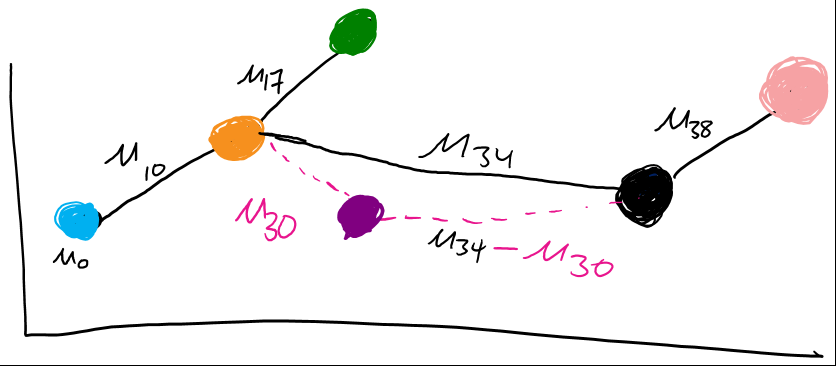
\includegraphics[width=0.5\textwidth]{figures/flipAndBalance}
	\caption{\textbf{Proposal 2 - Flip indicator and balance.} 
In this antigenic map, the purple cluster represents the new cluster of viruses generated by flipping $I_{30}$ from 0 to 1. In order to retain the absolute location of viruses in the black and pink clusters,  $\mu_{34}$ is adjusted by the value of $\mu_{30}$.
	} 
	\label{flipAndBalance} 
\end{figure}


The second class of proposals aims to improve MCMC mixing.
Proposal 3 switches status between a randomly chosen active $I_i$ with another randomly chosen inactive $I_i$. 
Unlike proposal 2, substituting an active node by another does not come with the penalty associated with increasing the number of active nodes.
Thus, proposal 3 could easily be accepted when it swaps a less ideal node with a node that have high evidence to be associated with antigenic transition.

Proposal 4 (Figure~\ref{multistep}) also performs a node substitution operation but swaps both the values of $I_i$ and $\mu_i$ of a randomly chosen active node $i$ with a node $j$ chosen from a small neighborhood around node $i$ in the phylogeny. 
This proposal is designed to suggest refinement to where a currently inferred cluster transition should be, given that the current suggestion is in node $i$.
As a refinement proposal, node $j$ also inherits the value of $\mu_i$, because when designing this proposal, we learned that swapping $\mu$ substantially improves the chance of accepting the move.
However, instead of naively using the current value of $\mu_j$, which can be any magnitude and direction, this proposal inherits the current value of  $\mu_i$, which is beneficial because this value is likely already near the optimal value of antigenic change.
Precisely, an active ($I_i=1$) node $i$ is chosen at random.
Then, the proposal identifies the list of $n_{c}$ nodes that are within a small neighborhood of node $i$ (i.e.  within 3 branches from node $i$ but excluding node $i$).
The proposal randomly picks a node $j$ within the list of candidates with equal probability $\frac{1}{n_{c}}$.
The proposal then swaps the value of $I_i$ by $I_j$ and the value of $\mu_i$ by $\mu_j$.

%This proposal has two desirable properties:
%First, swapping $I$ with a neighbor is much more efficient than swapping $I$ between two arbitrarily far nodes (as in no.3) because the former proposal makes a much smaller change to the virus partitioning than the latter proposal.
%Second, by also swapping $\mu$, the new active neighbour gets the value of $\mu_i$ from the now inactive pivot, so the virus assignment but not the cluster locations change. 

%From our experiment, we learned that swapping $\mu$ allows much higher observed acceptance rate ($3.2\%$) than not swapping $\mu$ ($1.1\%$), so we decided to includes swapping $\mu$ in proposal no.4.


%%% Illustration of the swap with neighbor proposal %%%
\begin{figure}[h]
	\centering		
	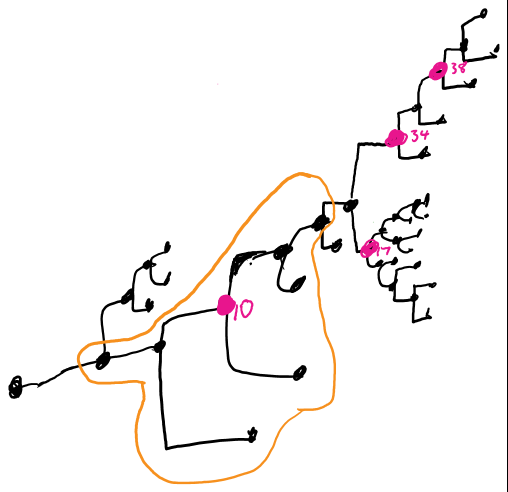
\includegraphics[width=0.5\textwidth]{figures/multistep}
	\caption{\textbf{Proposal 4 - Swap $I_i$ and $\mu_i$ with a neighbor} 
In this $T$, node 10 is chosen to perform the swap-with-neighbor proposal. In this case, with a neighborhood step-size of 2, the set of candidates are all the nodes within the orange neighborhood minus node 10.
	} 
	\label{multistep} 
\end{figure}



Proposal 5 selects a random dimension of a randomly chosen $\mu_i$ from an active node to perform a random walk while keeping the absolute location of other clusters fixed (Figure~\ref{walkAndBalance})
This proposal is designed to effectively sample the posterior distribution of $\mu_i$ of an active node. 
\begin{equation}
	\mu_i^{*} =  \mu_i + \delta \\
\end{equation},
where $\delta \sim \frac{1}{2} (U(-M, M), 0)' + \frac{1}{2} (0, U(-M, M))'$ and $M$ is the walk size learned initially by the adaptive MCMC scheme used in BEAST.
Similar to proposal 2, this proposal performs a balancing move on the antigenic map by
\begin{equation}
	\mu_j^{*} =  \mu_j - \delta\\     ,
\label{balance_mu}
\end{equation}
for each $j$ that is an active child node (i.e. $I_j = 1$) of node $i$.



%%% Illustration of the walk an active mu and balance proposal%%%
\begin{figure}[h]
	\centering		
	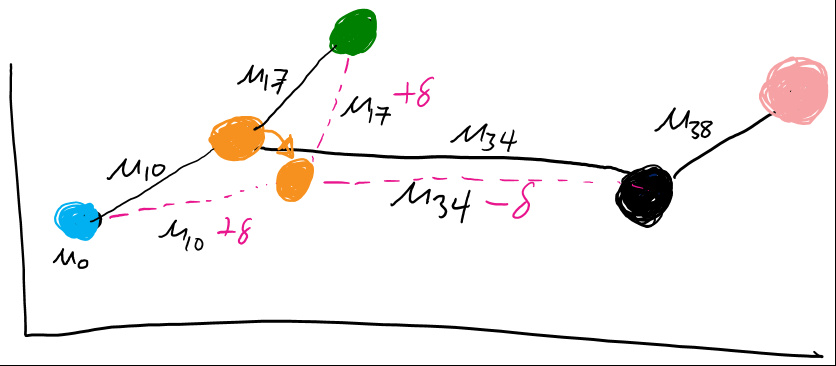
\includegraphics[width=0.5\textwidth]{figures/walkAndBalance}
	\caption{\textbf{Proposal 5 - Performs a random walk on an active $\mu_i$ and balance other active $\mu$'s.} 
In this antigenic map, $\mu_{10}$ is now changed by $\delta$, which causes the antigenic location of viruses in the orange cluster to change. 
To retain the absolute location of viruses in other clusters,  $\mu_{17}$ and $\mu_{34}$ are adjusted by subtracting $\delta$. [typo?  $\mu_{17} - \delta$, not +].
	} 
	\label{walkAndBalance} 
\end{figure}


%There are three reasons why we included this proposal.
This proposal is sensible for two reasons.
First, in contrast to proposal 1, here this proposal only focuses on the active nodes, nodes in which their $\mu$ directly influence the antigenic likelihood.
Instead of proposing from the prior, this proposal performs a random walk.
When the selected node $i$ is active, $\mu_i$ tends to prefer to be in a specific region, so sampling via random walk should be a more effective sampling strategy than sampling via independent proposal.
Our empirical evidence (not shown) also suggests that performing a random walk on active node dramatically improves the acceptance rate than sampling from an independent prior proposal.
Second, similar to proposal 1, empirical evidence (not shown) suggests that balancing the other $\mu$ substantially increases the chance of acceptance, mainly by preserving the relationship between viruses and sera in the antigenic map.
%random walk operator has dramatically higher chance of acceptance (16.4$\%$) than sampling from independent prior proposal ($0.x\%$).
%Second, by balancing the active $\mu$'s of the children clusters, we increase the chance of acceptance ( equation \ref{flipI_equation} + \ref{muBalance-equation} = 26.1$\%$ vs. equation \ref{flipI_equation} only =16.4$\%$).


The third class of proposals are situational because at least in theory they may help with MCMC mixing in some situations.
Proposal 6 modifies Proposal 2. 
This proposal is designed to increase the acceptance probability of Proposal 2. 
Recall that flipping a node causes the descending viruses to form a new cluster from their parent cluster.
If the variance of the prior for $\mu_i$ ($\sigma^2_u$) is large, $\mu_i$ would tend to be farther away from the origin. 
Then, unless the current $\mu_i$ is optimal, the change will likely negatively affect the posterior.  
A proposal that has higher chance of acceptance would simply be to only consider nodes with small $\mu_i$, so turning this node on will result in a birth of cluster that is close to its parent cluster.
To implement this idea, proposal 6 only considers a node as a candidate to be chosen randomly if its current value of $\mu_i$ is close to the origin (e.g. $ || \mu_i ||_2  < 2$).


Proposal 7 combines proposal 4 with flipping the indicator of a neighboring node. 
This proposal is designed to potentially replace one active node by two to form two subclusters, or vice versa.
The swap step is the same as that in proposal 4.
In the flip step, the proposal searches for the union of the neighbors from the existing node and the neighbors from the new node.
Taking the union of the sets allows a backward move to be always possible.
Each of the node in this union set has an equal chance to be selected (Figure~\ref{jointMultistep}).


%%% Illustration of the swap with a neighbor and flip another neighbor proposal%%%
\begin{figure}[h]
	\centering		
	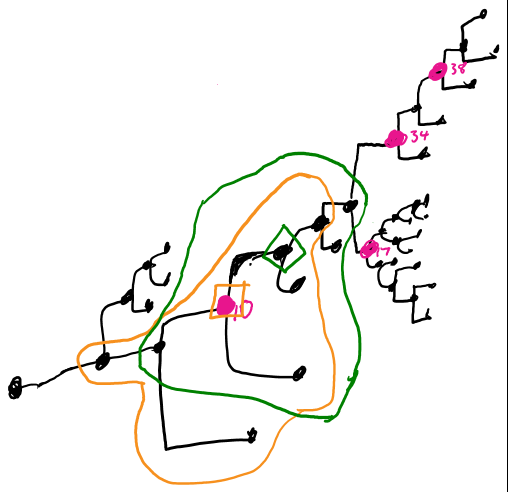
\includegraphics[width=0.5\textwidth]{figures/jointMultistep}
	\caption{\textbf{ The candidate of nodes to be flipped in Proposal 7 - Swap with a neighbor and flip another neighbor.} 
In the second operation that flips the indicator status of another neighbor, the list of nodes to consider include neighbors from the original pivot node and the neighbors of the newly chosen node. 
%Taking the union of the two set of nodes allows a node that may be further away to be chosen and also ensures that the  log Metropolis-Hasting ratio would be greater than 0 because the backward operation from the new state to the old state would also have a probability greater than 0.
	} 
	\label{jointMultistep} 
\end{figure}

%  [perhaps further explain the motivating example: the 604 $<-->$ 605, 592 situation]



To sample other parameters in the model, we used proposals inherited from the previous work \cite{bedford_integrating_2014}. 
There is one exception.
As described earlier, the Diffusion prior of the sera locations \cite{bedford_integrating_2014} spreads the first dimension of sera location across the antigenic map by sera dates ($d_i$) linearly by the serum drift term ($\beta$).
If a new $\beta^{*}$ is sampled via a scaled operator \cite{bedford_integrating_2014} by scaling the original value $\beta$, all the antigenic locations of sera change.
This change is potentially problematic because it affects the relationship between all viruses and sera on the antigenic map.
To minimize the impact of this change, we propose to couple this move with scaling the first dimension of $\mu_i$  proportionally, for each active node $i$. Precisely, 
\begin{equation}
\label{scaleMu1}
 \mu_{i1}^* = \mu_{i1} \frac{ \beta^*}{\beta} .
\end{equation}



We implemented our clustering method in BEAST v1.8.0 and is available for download at http://BEAST.
MCMC outputs are summarized in tables and parameters that are associated with the tree (eg. cluster labels, antigenic change, virus location) are also integrated into the output NEXUS-formatted phylogenetic tree file to enable convenient visualization in FigTree \cite{FIGTREE}.





%The first proposal (no.6) is a companion of proposal no. 4. 
%In a separate routine, we first record the frequency of which the MCMC chain accepts a change in $I$ and updates this list in every user-defined (e.g. 100,000) number of steps from all other proposals.
%The set of nodes that are called accepted are called the "hot" nodes. 
%Proposal no.6 is identical to proposal no.4 except that only the "hot" nodes can be candidates to swap to. 
%By limiting the number of nodes to consider, this proposal has shown to be accepted up to 4 times more than proposal no. 4 when $p$ is set to be very small (p=0.001?), likely because in this situation a new indicator does not get accepted very often?? (think more why!)
%[For simplicity, we decided not to use this proposal unless p is small, because under the default $p=0.02$, the improvement was not too substantial.]



%serumDriftActiveScaledMu1Operator


% We used a random walk operator that is similar to that in equation \ref{muBalance-equation} to explore the space each $Y_i$. 




\subsection*{Materials}

%Need paraphrase

In the analysis of real data, we used antigenic datasets \cite{bedford_integrating_2014} of HI measurements of virus isolates against post-infection ferret sera for A/H3N2 and A/H1N1 collected and compiled from publications \cite{Smith04,Kendal78,Webster79,Nakajima79,Nakajima81,Chakraverty82,Pereira82,Chakraverty86,Cox83,Daniels85,Raymond86,Stevens87,Donatelli93,Hay01,Daum02,McDonald07,Barr10}
The A/H3N2 dataset consists of 402 virus isolates, 519 serum isolates, with a total of 10,059 HI measurements from 1968 to 2011. 
The A/H1N1 dataset consists of 115 virus isolates, 77 serum isolates, with a total of 1882 HI measurements from 1977 to 2009.
Other details of the datasets were described in a previous work \cite{bedford_integrating_2014}.

We obtained HA nucleotide sequences for A/H3N2 and A/H1N1 from a previous study \cite{bedford_integrating_2014} that collected the data from the Influenza Research \cite{IRD} and the EpiFlu databases \cite{GISAID}. 
First, these databases were queried by matching strain names, e.g.\ A/HongKong/1/1968, that corresponded with the strain names from the antigenic datasets.
Second, sequences were aligned by using MUSCLE v3.7 under default settings \cite{MUSCLE}.
Third, BEAST\cite{BEAST17} was used to perform phylogenetic inference on the A/H3N2 and A/H1N1 datasets.
In these analyses, the SRD06 nucleotide substitution model \cite{Shapiro06}, a coalescent demographic model with constant effective population size and a strict molecular clock across branches, was used.
The MCMC sampled 60 million steps and every 50,000th steps was printed.
Allowing for a burn-in of 10 million steps, a total sample of 2000 trees were kept for subsequent clustering analysis.
Finally, for each analysis, we generated the MCC tree by using TreeAnnotator version 1.8.0.





\subsection*{Analysis of the A/H3N2 and A/H1N1 Datasets}

	
%mds precision level... use  symbol.. phi to represent
We performed antigenic clustering using the antigenic data and the MCC tree from the A/H3N2 and A/H1N1 datasets. 
Recall that the MDS precision is a tuning parameter used to control how much measurement noise is tolerated within a cluster, with higher value promoting the detection of more clusters. 
After some initial tests, we considered the $\kappa$ at 0.05, 0.1, and 0.15 for A/H3N2 and 0.1 and 0.3 for A/H1N1 that give sensible number of detected viral clusters.  
Each MCMC was run for 500 million steps and trees were sampled at every 200,000 steps. 
Allowing for a burn-in of 50 million steps, a total of 2001 samples were kept.
We summarized the MCMC outputs by several ways. 
First, we used FigTree v1.4.2 to visualize clusters across different  MCMC samples. 
Second, we plotted the antigenic maps of different samples and annotated the viral clusters with path of antigenic transitions. 
Third, we produced heatmaps to summarize the variation in our probabilistic cluster assignment. 
For direct correspondence to the phylogenetic tree displayed in FigTree, the viruses were sorted by the order as appeared in the FigTree.
Heatmap is a very useful summary of clustering because it ultimately captures the probability that each pair of virus shares the same clusters, hence visually presenting the major clustering patterns among all viruses, even when the exact transition branch cannot be inferred with high confidence. %a sentence about why heatmap is highly appropriate 
Fourth, we performed convergence analysis by (1)inspecting convergence diagnostic plots of MCMC outputs generated by Tracer v1.5, (2)comparing across replicates the probabilities that each node is active, which collectively are the main parameters of interest, and (3)computing the Gelman-Rubin statistics on these parameters. 
The probability that node $i$ is active ($p_i$) is computed by taking the average of the realized samples of $I_i$ (i.e. $I_i^b$, for $b=1,...B$), where $B$ is the number of stored MCMC samples.
\begin{equation}
 \hat{p_i} = \frac{1}{N} \sum_{b=1}^{B} I(I_i^b  = 1).
\end{equation}
Finally, we evaluated the impact of using different inferred tree topologies instead of the MCC tree. 
We performed antigenic clustering by using different MCMC sampled trees (iteration 20, 30, 40, 50, and 60 million) and compared the results using heatmaps.
The results are available for download at http://github....


\subsubsection*{Evaluation of Antigenic Clustering via Simulation}


% rediscovering clusters via simulations.

To evaluate the clustering method, we simulated clusters on viruses and antigenic data based on viruses from the more computationally challenging A/H3N2 phylogeny.
Step 1 generates 15 active nodes on the MCC tree. 
In this procedure, a node is added one at a time from the set of remaining inactive nodes.
At each step, a random node is added to the set of active nodes.
This node is added to the set of active nodes only if the phylogeny is partitioned in a way such that the smallest cluster has at least 10 viruses. 
Otherwise, this step is repeated until the candidate node satisfies this minimum size condition.
At the end, the set of active nodes generates a total of 16 clusters each with a minimum cluster size of 10 viruses.
This number of clusters is in the range of the number of previously inferred clusters for A/H3N2\cite{smith_mapping_2004}. 
Step 2 simulates the antigenic data.
Five sera are simulated for each cluster to produce a total of 80 sera, which is considerably smaller than the number of sera (519) from the real data for A/H3N2, but it already had enough information for the inference.
For each virus $i$ and serum $j$, the log$_2$ observed titer was simulated from 
\begin{equation}
 \label{simulationEquation}
H_{ij} \sim N(  10 -  2 \omega(i,j) ,  \sigma^2 )     ,
\end{equation}
where $\omega_{ij}$ is a distance function that calculates the number of cluster transitions  between virus $i$ and the reference virus of serum $j$ on the phylogeny.
Equation (\ref{simulationEquation}) models the realistic scenario that the strength of reactivity between virus $i$ and serum $j$ decreases as the number of major cluster transitions between virus $i$ and the reference virus in serum $j$ increases.
For example, the expected log$_2$ titer for virus $i$ and serum $j$ with reference virus from the same cluster is 10, while the expected log$_2$ titer for virus $i$ and serum $j$ with reference virus from a cluster separated by 2 cluster transitions is 6.
$\sigma^2 = 1$ is used to model the scenario that a log$_2$ titer measurement has a nontrivial amount of measurement noise (Figure \ref{SimulationNoise}) around its expected titer value.
In addition, the date (in year) of each serum was simulated because it is required by the Diffusion prior for serum.
Because it is reasonable to assume that each serum is made from a virus in the phylogeny, the simulation draws a random sample from the list of dates of viruses in the cluster to be the date of a serum in that cluster.
Step 3 generates missing data from the complete matrix of antigenic data to approximate the reality that our datasets often contain missing data.
The thinning procedure uses a random number generator to decide whether to keep each of the 32,160 observations from the original dataset.
Thinning is performed on varying levels to evaluate the impact of data completion rate, with approximately 50\%, 20\%, 10\%, and 5\% of observations retained from the original dataset.
We repeated these steps to obtain 5 independent simulations.

%maybe put in the Supplementary Materials
\begin{figure}[h]
	\centering		
	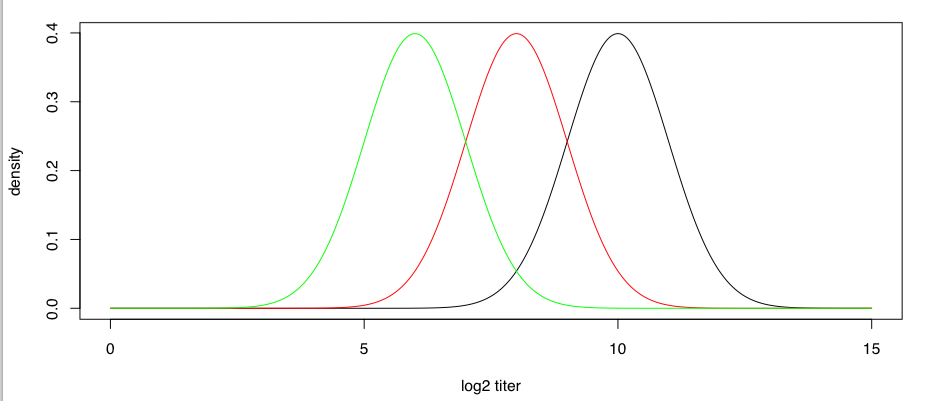
\includegraphics[width=0.7\textwidth]{figures/custom/simulationNoise}
	\caption{\textbf{Simulation of log$_2$ HI titer consists of measurement noises.} 
	 For a virus $i$ and a reference virus for serum $j$ that belongs to the same antigenic cluster, the distribution of measurements follows $N(10, \sigma^2)$. For each antigenic transition between the two viruses, the mean measurement decreases by 2 units.	
	 		} 
	\label{SimulationNoise} 
\end{figure}



We then evaluated our clustering method.
First, we performed antigenic clustering on each simulated dataset.
We ran each analysis for 50 million MCMC iterations and printed every 50,000th iteration.
With the first 10\% of outputs used as burn-ins, each analysis consists of $B=901$ samples.
Second, we estimated $p_i$ for each $i$.
Third, for each degree of data completion rate, we averaged the results over replicates and plotted the Receiver Operating Curve (ROC) of true positives vs. false positives as a function of detection threshold ($\lambda$), which is the probability threshold used in calling a node significant.
Sensitivity is defined as the percent of true positives inferred, averaged over replicates. By default, $\lambda=0.5$ was used as the threshold for detection.
%heatmap?







\newpage

%%% REFERENCES %%%

%need to check for redundancy, since I am using two sources that sometimes cite the same paper
\bibliographystyle{plos}
\bibliography{flux,citations}

\end{document}




\newpage

